
\documentclass[../notes.tex]{subfiles}

\graphicspath{{\subfix{../img/}}}

\begin{document}

\section{ECE353 Operating Systems}

\begin{blockquote}
    Examples and some figures taken from Prof. Jon Eyolfson's ECE353 slides and notes (https://eyolfson.com).
\end{blockquote}


\subsection{Kernel Mode}
\subsubsection{ISAs and Permissions}

There are a number of ISAs in use today; x86 (amd64), aarch64 (arm64), and risc-v are common ones.
For purposes of this course we will study largely arm systems but will touch on the other two as well.

\begin{figure}[H]
  \centering
  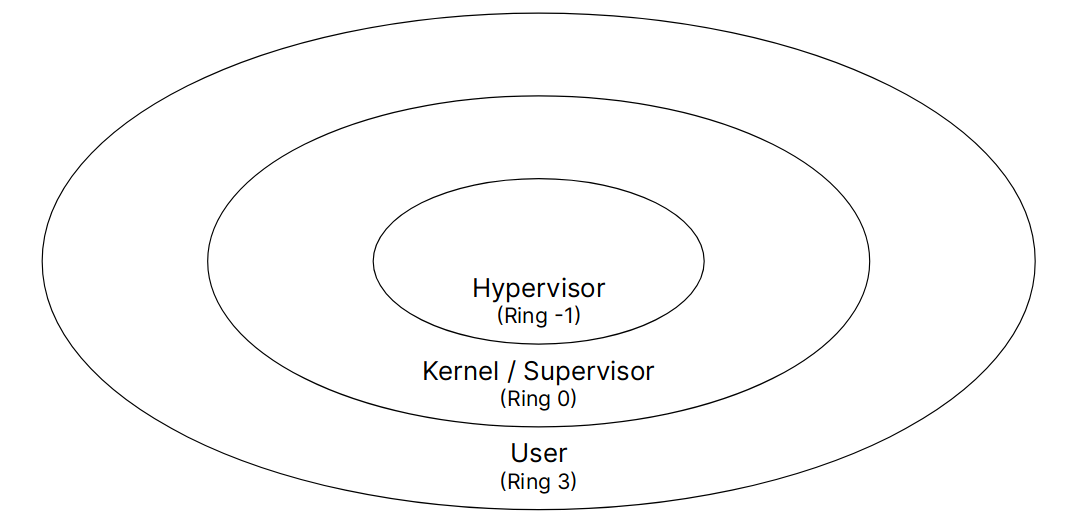
\includegraphics[width=0.8\linewidth]{img/image_2023-01-11-15-18-10.png}
  \caption{x86 Instruction access rings. Each ring can access instructions in its outer rings.}
\end{figure}

The kernel runs in, well, Kernel mode. \textbf{System calls} offer an interface between user and kernel mode\mn{Linux has 451 total syscalls}. 

\marginnote{Note: API (application programming interface), ABI (Application Binary Interface). API abstracts communication interface (i.e. two ints), ABI is how to layout data, i.e. calling convention}

The system call ABI for x86 is as follows:

\begin{figure}[H]
  \centering
  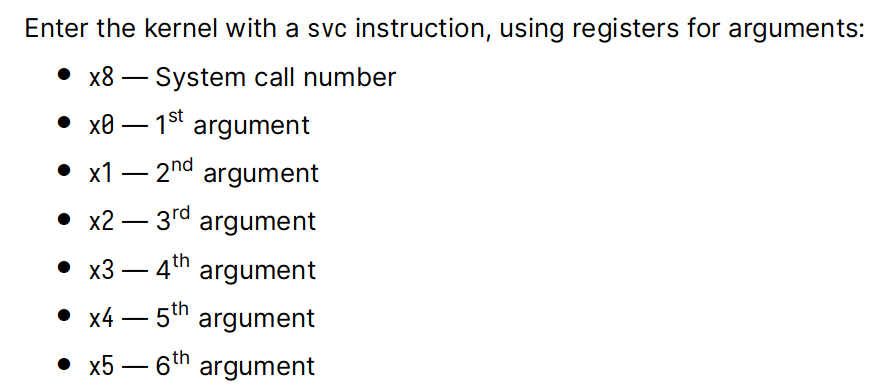
\includegraphics[width=0.8\linewidth]{img/image_2023-01-11-15-23-26.png}
\end{figure}

This ABI has some limitations; i.e. all arguments must be a register in size and so forth, which we generally circumvent by using pointers.

For example, the \texttt{write} syscall can look like:


\begin{listing}[H]
\begin{minted}{c}
ssize_t write(int fd, const void* buf, size_t count);
// writes bytes to a file descriptior
\end{minted}
\end{listing}


\subsubsection{ELF (Executable and Linkable Format)}


\begin{itemize}
  \item  Aways starts with 4 bytes: \texttt{0x7F, 'E', 'L', 'F'}
  \item Followed byte for 32 or 64 bit architecture
  \item Followed by 1 byte for endianness
\end{itemize}
\marginnote{Most file formats have different starting signatures or magic numbers}

\texttt{readelf} can be used to read \texttt{ELF} file headers.

For example, \texttt{readelf -a \$(which cat)} produces (output truncated)



\begin{listing}[H]
\begin{minted}{text}
ELF Header:
  Magic:   7f 45 4c 46 02 01 01 00 00 00 00 00 00 00 00 00
  Class:                             ELF64
  Data:                              2's complement, little endian
  Version:                           1 (current)
  OS/ABI:                            UNIX - System V
  ABI Version:                       0
  Type:                              DYN (Position-Independent Executable file)
  Machine:                           Advanced Micro Devices X86-64
  Version:                           0x1
  Entry point address:               0x32e0
  Start of program headers:          64 (bytes into file)
  Start of section headers:          33152 (bytes into file)
  Flags:                             0x0
  Size of this header:               64 (bytes)
  Size of program headers:           56 (bytes)
  Number of program headers:         13
  Size of section headers:           64 (bytes)
  Number of section headers:         26
  Section header string table index: 25
\end{minted}
\end{listing}
\marginnote{This output is followed by information about the program and section headers}


\texttt{strace} can be used to trace systemcalls. For example let's look at the 168-byte hello-world example


\begin{listing}[H]
\begin{minted}{text}
0x7F 0x45 0x4C 0x46 0x02 0x01 0x01 0x00 0x00 0x00 0x00 0x00 0x00 0x00 0x00 0x00
0x02 0x00 0xB7 0x00 0x01 0x00 0x00 0x00 0x78 0x00 0x01 0x00 0x00 0x00 0x00 0x00
0x40 0x00 0x00 0x00 0x00 0x00 0x00 0x00 0x00 0x00 0x00 0x00 0x00 0x00 0x00 0x00
0x00 0x00 0x00 0x00 0x40 0x00 0x38 0x00 0x01 0x00 0x40 0x00 0x00 0x00 0x00 0x00
0x01 0x00 0x00 0x00 0x05 0x00 0x00 0x00 0x00 0x00 0x00 0x00 0x00 0x00 0x00 0x00
0x00 0x00 0x01 0x00 0x00 0x00 0x00 0x00 0x00 0x00 0x01 0x00 0x00 0x00 0x00 0x00
0xA8 0x00 0x00 0x00 0x00 0x00 0x00 0x00 0xA8 0x00 0x00 0x00 0x00 0x00 0x00 0x00
0x00 0x10 0x00 0x00 0x00 0x00 0x00 0x00 0x08 0x08 0x80 0xD2 0x20 0x00 0x80 0xD2
0x81 0x13 0x80 0xD2 0x21 0x00 0xA0 0xF2 0x82 0x01 0x80 0xD2 0x01 0x00 0x00 0xD4
0xC8 0x0B 0x80 0xD2 0x00 0x00 0x80 0xD2 0x01 0x00 0x00 0xD4 0x48 0x65 0x6C 0x6C
0x6F 0x20 0x77 0x6F 0x72 0x6C 0x64 0x0A
\end{minted}
\caption{Note: This is for arm cpus}
\end{listing}


If we run this then we see that the program makes a \texttt{write} syscall as well as a \texttt{exit\_group}

\begin{listing}[H]
\begin{minted}{text}
execve (" ./ hello_world " , [ " ./ hello_world " ] , 0 x7ffd0489de40 /* 46 vars */ ) = 0
write (1 , " Hello world \ n " , 12) = 12
exit_group (0) = ?
+++ exited with 0 +++
\end{minted}
\end{listing}

Note that these strings are not null-terminated (null-termination is just a \texttt{c} thing) because we don't want to be unable to write strings with the null character to it.


\begin{figure}[H]
  \centering
  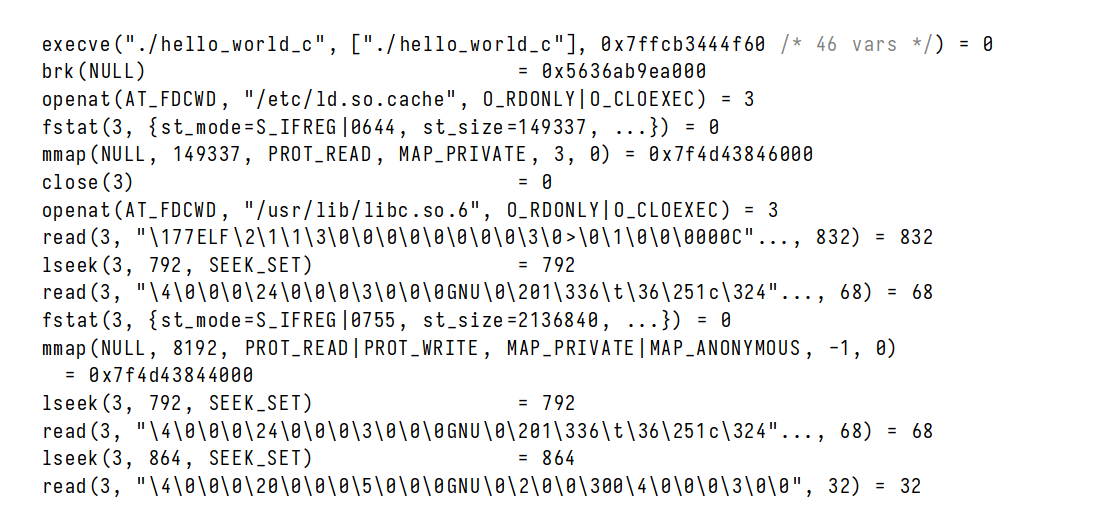
\includegraphics[width=0.8\linewidth]{img/image_2023-01-11-15-48-48.png}
  \caption{A c hello world would load the stdlib before printing...}
\end{figure}


\subsubsection{Kernel}
The kernel can be thought of as a long-running program with a ton of library code which executes on-demand. Monolithic kernels run all OS services in kernel mode, but micro kernels run the minimum amount of servers in kernel mode. Syscalls are slow so it can be useful to put things in the kernel space to make it faster. But there are security reasons against putting everything in kernel mode.


\subsubsection{Processes \& Syscalls}

A process is like a combination of all the virtual resources; a "virtual GPU" (if applicable), memory (addr space), I/O, etc.
The unique part of a struct is the PCB (Process Control Block) which contains all of the execution information. In Linux this is the \texttt{task\_struct} which contains information about the process state, CPU registers, scheduling information, and so forth.


\begin{figure}[H]
  \centering
  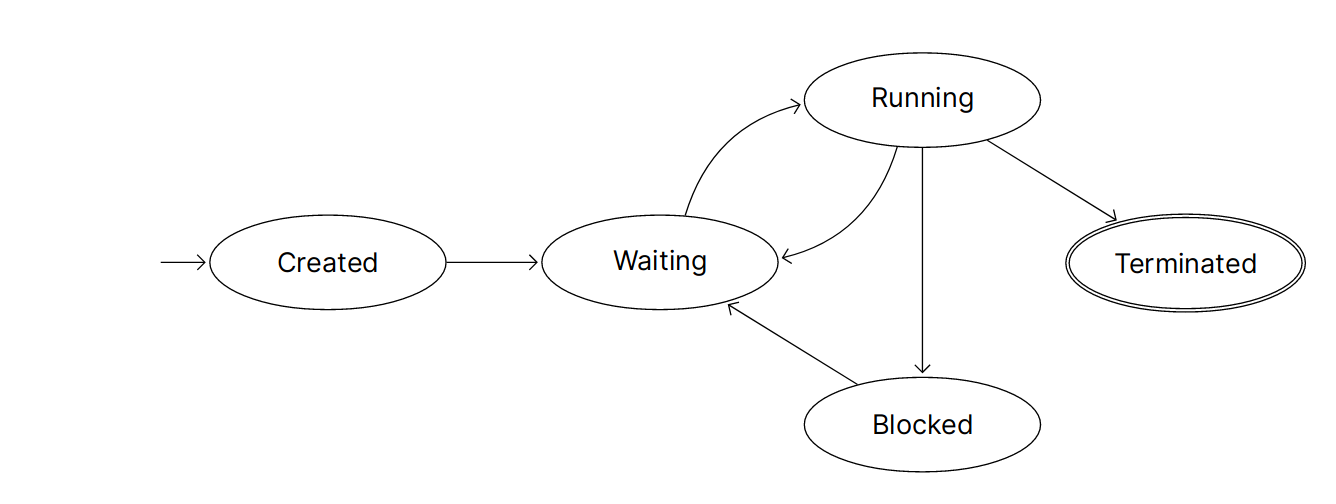
\includegraphics[width=0.8\linewidth]{img/image_2023-01-12-15-21-01.png}
  \caption{A possible process state diagram}
\end{figure}

These state changes are managed by the Process and OS\mn{I think} so that the OS scheduler can do its job.
An example of where some of these states can be useful would be to free up CPU time while a process is in the Blocked state while waiting for IO.
Process can either manage themselves (cooperative multitasking) or have the OS manage it (true multitasking).
Most systems use a combination of the two, but it's important to note that cooperative multitasking is not true multitasking.

\marginnote{Process state can be read in \texttt{/proc} for linux systems. }


Context switching (saving state when switching between processes) is expensive. Generally we try to minimize the amount of state that has to be saved (the bare minimum is the registers).
The scheduler decides when to switch. Linux currently uses the CFS\mn{completely fair scheduler}.


In \texttt{c} most system calls are wrapped to give additional features and to put them more concretely in the userspace.


\begin{figure}[H]
  \centering
  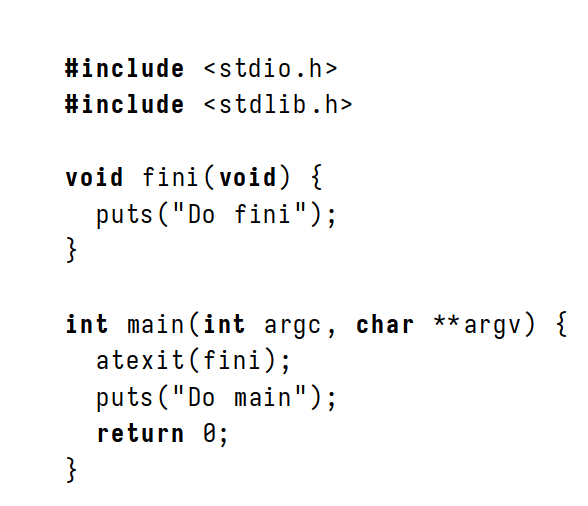
\includegraphics[width=0.8\linewidth]{img/image_2023-01-12-15-34-58.png}
  \caption{Demonstration of c feature to register functions to call on program exit}
\end{figure}

\begin{listing}[H]
\begin{minted}{c}
int main ( int argc , char * argv []) {
  printf ("I 'm going to become another process \n" );
  char * exec_argv [] = {" ls " , NULL };
  char * exec_envp [] = { NULL };
  int exec_return = execve ("/ usr / bin / ls " , exec_argv , exec_envp );
  if ( exec_return == -1) {
    exec_return = errno ;
    perror (" execve failed " );
    return exec_return ;
  }
  printf (" If execve worked , this will never print \n" );
  return 0;
}
\end{minted}
\caption{Demo of execve turning current program to ls (executes program, wrapper around exec syscall)}
\end{listing}

\begin{listing}[H]
\begin{minted}{c}
#include <sys/syscall.h>
#include <unistd.h>

int main (){
  syscall(SYS_exit_group, 0);
}

\end{minted}
\caption{An example of using a raw syscall system exit instead of c's exit()}
\end{listing}

\subsection{Fork, Exec, And Processes}

\begin{itemize}
    \item \texttt{fork} creates a new process which is a copy of the current process. Everything is exactly the same except for the PID in the child and PID in the parent.
        \begin{itemize}
            \item Returns -1 on error, 0 in the child process, and the pid of the child in the parent process
        \end{itemize}
    \item \texttt{exec} replaces the current process with a new one
        \begin{itemize}
            \item Returns -1 on error
        \end{itemize}


\end{itemize}

Process states:

\begin{itemize}
    \item The CPU is responsible for \textit{scheduling} processes, so there can be >1 process per core.
    \item Maintaining the parent-child relationship
        \begin{itemize}
            \item Parent is responsible for the child 
            \item This usually works; the parent can wait for the child to finish. But what if the parent crashes, etc?
            \item Zombie: a process that has finished but has not been cleaned up by its parent. This can be a problem because the process is still using resources. The OS has to keep a zomibe process until it's acknowledged. To avoid zombie build-up the OS can signal the parent process (over IPC) to acknowledge the child. (The parent can ignore it)
            \item Orphan: a process that has no parent. This can happen if the parent crashes. The OS can adopt the orphan and make it a child of the init process which can keep onto them or kill them as needed.
        \end{itemize}
\end{itemize}

\begin{listing}[H]
\begin{minted}{c}
int main(int argc, char *argv[]) {
    pid_t pid = fork();
  if (pid == -1) {
    int err = errno; perror("fork failed"); return err;
  }
  if (pid == 0) {
    printf("Child parent pid: %d\n", getppid());
    sleep(2);
    printf("Child parent pid (after sleep): %d\n", getppid());
  }
  else {
    sleep(1); }
  return 0; }
\end{minted}
\caption{orphan example: parent exits before child and \texttt{init} has to clean up}
\end{listing}

\subsection{IPC}

Reading and writing files is a form of IPC. For example, a simple process could write everything it reads, i.e this facsimile of the \texttt{cat} program

\marginnote{Standard file descriptors: 0 = stdin, 1 = stdout, 2 = stderr}

\begin{listing}[H]
\begin{minted}{c}
int main() {
  char buffer[4096];
  ssize_t bytes_read;
  // read (see man 2 read) reads from a file descriptor
  // can't assume always successful; see from `man errno`
  //   Nearly all of the system calls provide an error number in the external variable errno, which is defined as: extern int errno. Refer to man pages for what each errno means.

  while ((bytes_read = read(0, buffer, sizeof(buffer))) > 0) {
    ssize_t bytes_written = write(1, buffer, bytes_read);
    if (bytes_written == -1) {
      int err = errno;
      perror("write");
      return err;
    }
    assert(bytes_read == bytes_written);
  }
  if (bytes_read == -1) {
    int err = errno;
    perror("read");
    return err;
  }
  assert(bytes_read == 0);
  return 0;
}
\end{minted}
\end{listing}


Another way of IPC is using signals. Common signals include

\begin{itemize}
    \item SIGINT (Ctrl-C)
    \item SIGKILL (kill -9)
    \item EOF (Ctrl-D)
\end{itemize}


A signal pauses (interrupts) your program and then runs the signal handler. Process can be interrupted at any point in execution, and the process will resume after the signal handler finishes.


\begin{listing}[H]
\begin{minted}{c}
void handle_signal(int signum) {
  printf("Ignoring signal %d\n", signum);
}

void register_signal(int signum)
{
  struct sigaction new_action = {0};
  sigemptyset(&new_action.sa_mask);
  new_action.sa_handler = handle_signal;
  if (sigaction(signum, &new_action, NULL) == -1) {
    int err = errno;
    perror("sigaction");
    exit(err);
  }
}

\end{minted}
\end{listing}

// breaking here

\begin{listing}[H]
\begin{minted}{c}

int main(int argc, char *argv[])
{
  if (argc > 2) {
    return EINVAL;
  }

  if (argc == 2) {
    close(0);
    int fd = open(argv[1], O_RDONLY);
    if (fd == -1) {
      int err = errno;
      perror("open");
      return err;
    }
  }

  register_signal(SIGINT);
  register_signal(SIGTERM);

  char buffer[4096];
  ssize_t bytes_read;
  while ((bytes_read = read(0, buffer, sizeof(buffer))) > 0) {
    ssize_t bytes_written = write(1, buffer, bytes_read);
    if (bytes_written == -1) {
      int err = errno;
      perror("write");
      return err;
    }
    assert(bytes_read == bytes_written);
  }
  if (bytes_read == -1) {
    int err = errno;
    perror("read");
    return err;
  }
  assert(bytes_read == 0);
  return 0;
}
\end{minted}
\end{listing}

\begin{itemize}
    \item \texttt{register\_signal} sets a bunch of things such that we can handle the signal i.e. execute a function when a signal occurs. In this program we register SIGINT and SIGTERM with the kernel to execute \texttt{handle\_signal}. 
    \item This will still fail on ctrl-c because the read system call can error out
\end{itemize}


\begin{listing}[H]
\begin{minted}{c}
ssize_t bytes_read;
  while ((bytes_read = read(0, buffer, sizeof(buffer))) != 0) {
    if (bytes_read == -1) {
      if (errno == EINTR) {
	continue;
      }
      else {
	break;
      }
    }
    ssize_t bytes_written = write(1, buffer, bytes_read);
    if (bytes_written == -1) {
      int err = errno;
      perror("write");
      return err;
    }
    assert(bytes_read == bytes_written);
  }
  if (bytes_read == -1) {
    int err = errno;
    perror("read");
    return err;
  }
  assert(bytes_read == 0);
  return 0;
}
\end{minted}
\end{listing}

\begin{itemize}
    \item This snippet checks errno. and trys read again. Then the program is able to handle ctrl-c.
    \item This program can still get killed by kill -9 since it doesn't handle SIGKILL.
    \item Let's say we register $ SIGKILL $ with the kernel to execute \texttt{handle\_signal}. This will not work because you aren't allowed to ignore SIGKILL (-9).
\end{itemize}


Another thing we're interested in is to find out when a process is done. This can be polling on \texttt{waitpid}\mn{wait for process termination}

\begin{listing}[H]
\begin{minted}{c}

int main() {
  pid_t pid = fork();
  if (pid == -1) {
    return errno;
  }
  if (pid == 0) {
    sleep(2);
  }
  else {
    pid_t wait_pid = 0;
    int wstatus;

    unsigned int count = 0;
    while (wait_pid == 0) {
      ++count;
      printf("Calling wait (attempt %u)\n", count);
      wait_pid = waitpid(pid, &wstatus, WNOHANG);
    }

    if (wait_pid == -1) {
      int err = errno;
      perror("wait_pid");
      exit(err);
    }
    if (WIFEXITED(wstatus)) {
      printf("Wait returned for an exited process! pid: %d, status: %d\n", wait_pid, WEXITSTATUS(wstatus));
    }
    else {
      return ECHILD;
    }
  }
  return 0;
}
\end{minted}
\end{listing}

Alternatively, we should use interrupts
\marginnote{Note: interrupt handlers run to completion. But an interrupt handler may occur while another interrupt handler is running, so execution must be passable and state managed accordingly}

\begin{listing}[H]
\begin{minted}{c}
void handle_signal(int signum) {
  if (signum != SIGCHLD) {
    printf("Ignoring signal %d\n", signum);
  }


  printf("Calling wait\n");
  int wstatus;
  pid_t wait_pid = wait_pid = waitpid(-1, &wstatus, WNOHANG);
  // Here in our interrupt (signal) handler) we check for SIGCHILD and then waitpid the child if applicable
  if (wait_pid == -1) {
    int err = errno;
    perror("wait_pid");
    exit(err);
  }
  if (WIFEXITED(wstatus)) {
    printf("Wait returned for an exited process! pid: %d, status: %d\n", wait_pid, WEXITSTATUS(wstatus));
  }
  else {
    exit(ECHILD);
  }
  exit(0);
}


void register_signal(int signum) {
  struct sigaction new_action = {0};
  sigemptyset(&new_action.sa_mask);
  new_action.sa_handler = handle_signal;
  if (sigaction(signum, &new_action, NULL) == -1) {
    int err = errno;
    perror("sigaction");
    exit(err);
  }
}

int main() {
  register_signal(SIGCHLD);

  pid_t pid = fork();
  if (pid == -1) {
    return errno;
  }
  if (pid == 0) {
    sleep(2);
  }
  else {
    while (true) {
      printf("Time to go to sleep\n");
      sleep(9999);
    }
  }
  return 0;
}
\end{minted}
\end{listing}


On a RISC-5 CPU there are three terms for interrupts:

\begin{itemize}
    \item Interrupt: by external hardware and handled by kernel
    \item Exception: triggered by an instruction, kernel handles though process can optionally handle
    \item Trap: transfer of control of a trap handler by either an exception or interrupt. Syscall is a requested trap
\end{itemize}

\subsection{Pipe}

\begin{definition}
    \begin{listing}[H]
    \begin{minted}{c}
    int pipe(int pipefd[2]);
    \end{minted}
    \end{listing}

    Returns 0 on success, -1 on failure (and sets errno). Forms a one-way communication channel with 2 file descriptors; 0 for reading and 1 for writing. The pipe is unidirectional.

\end{definition}

\subsection{Basic Scheduling}

\begin{itemize}
    \item A pre-emptive resource can be taken and used for something else; i.e. CPU. Shared via scheduling
    \item A non-pre-emptive resource cannot be taken and used for something else; i.e. I/O. Shared via alloc/dealloc or queuing. Note that some parallel or distributed systems may allow you to allocate a CPU
    \item Dispatcher: responsible for context switching. Scheduler: deciding which processes to run
    \item Non-preemptible processes must run until completion, so the scheduler can only make a decision on termination.
    \item Pre-emptive allows the OS to run scheduler at will.
    \item Schedulers seek to minimize waiting time and maximize cpu utilization/throughput -- all while giving each process the same percent of CPU time.
\end{itemize}


\begin{definition}
    FCFS (First come first served) is a scheduling algorithm  that runs the process that arrives first. Processes are stored in a queue in arrival order. This has the downside of potentially introducing long wait times if longer tasks arrive before shorter ones.
\end{definition}

\begin{definition}
    SJF (Shortest job first): schedule the job with the shorts execution time first. Though it's optimal at minimizing average wait times, since we don't know how long each process takes it may not be practically optimal. It also has the downside of potentially starving longer jobs.
\end{definition}


\begin{definition}
    SRTF (Shortest Remaining Time First): schedule the job (with pre-emptions now) with the shortest remaining time. This optimizes the average waiting time.

    \begin{figure}[H]
        \centering
        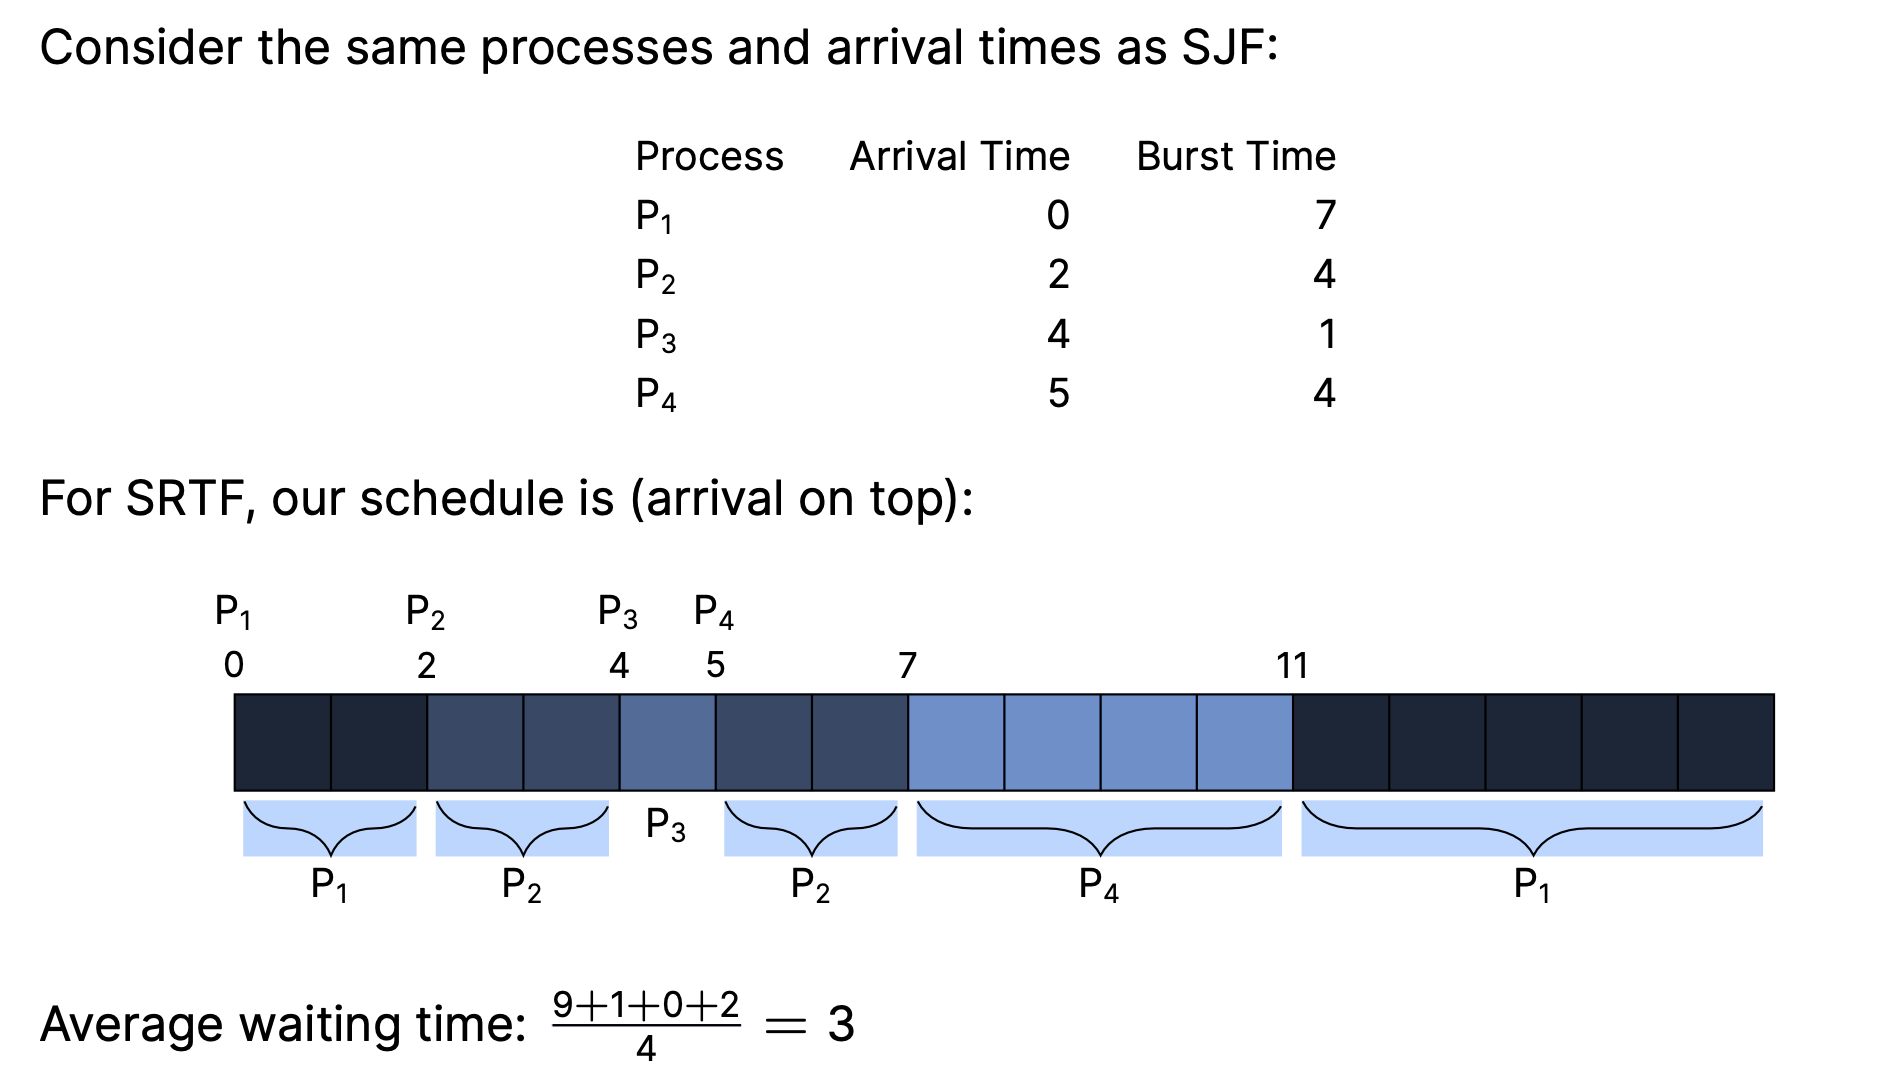
\includegraphics[width=0.8\linewidth]{img/image_2023-01-24-01-47-37.png}
    \end{figure}
\end{definition}


So far we haven't considered fairness. We can make a scheduler more fair by using a round-robin scheduler, which is a pre-emptive scheduler which divides execution time into quanta and gives processes <quanta> of time while round-robining through them. \mn{How to consider quantum length? Consider context switching time}

\begin{figure}[H]
    \centering
    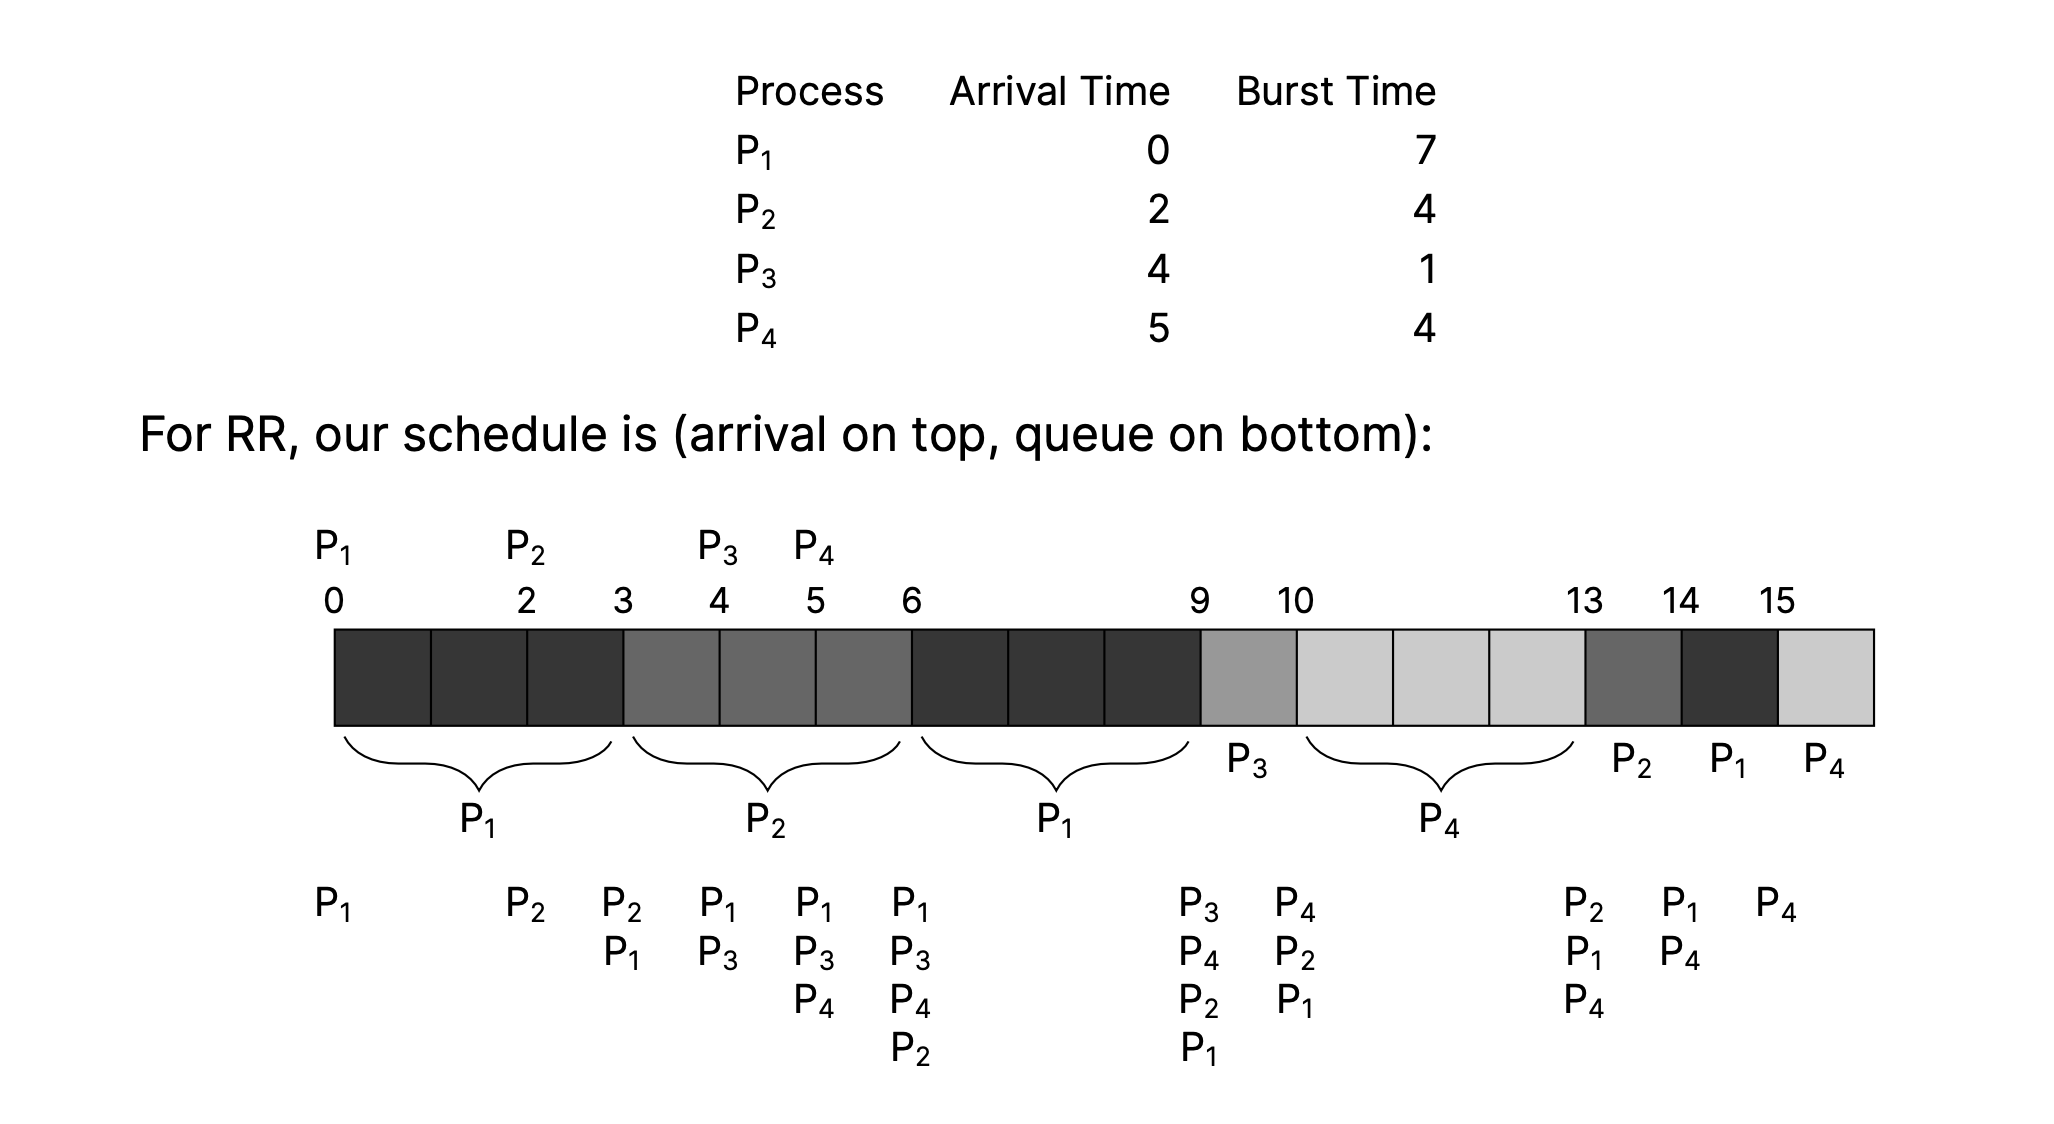
\includegraphics[width=0.8\linewidth]{img/image_2023-01-24-01-49-33.png}
    \caption{RR example with quanta of 3 units. Average number of switches is 7, average waiting time is $ \frac{8+8+5+7}{4} = 7 $, average response time is $ \frac{0 + 1 + 5 + 5 }{4}$. Note that ties are handled by favouring new processes.}
\end{figure}


Round robin performance is dependent on quantum length and job length. Long quantum causes starvation (FCFS), but twoo low and the performance sucks since context switches introduce overhead. 
If jobs have similar lengths RR has poor average waiting time

\subsection{Advanced Scheduling}

\begin{itemize}
    \item Processes can be given a priority. Linux: some integer value -20 -> 19
    \item Processes may \textit{starve} if there a lot of higher priority processes. Can be resolved by dynamically changing priorities i.e. upping priority of a old process
\end{itemize}

\begin{definition}
    \textbf{Priority inversion}: accidentally changing priority of low priority process to high through some dependency (i.e. high priority depending on low priority), which effectively flips the actual task priority.

    This is a problem and a common solution for it is \textit{priority inheritance}, where when a job blocks one or more high-priority jobs it ignores the original assessment and executes it's critical section\mn{The blocking portion} at a higher priority level, then returns to its original level.

\end{definition}


\begin{itemize}
    \item Recall: \texttt{fg}, \texttt{bg}, \texttt{ctrl-z}, \texttt{jobs}, and so forth
    \item Foreground/background processes foreground processes are those that are currently running and can be interacted with. Background processes are those that are running in the background and cannot be interacted with (take user input). This is to separate processes that need good response times nad those that don't.
        \marginnote{Formally UNIX background processes are ones where the process group ID differs from its terminal group ID}
    \item One strategy is to create different queues for foreground and background processes, i.e. round-robin forground and then FCFS for background ... then schedule between the queues
\end{itemize}


Scheduling is a complex topic and there are many more algorithms that make an array of tradeoffs


\subsection{Symmetric Multiprocessing (SMP)}

\begin{definition}
    \textbf{Symmetric Multiprocessing}:

\begin{itemize}
    \item All CPUS connected to same physical memory
    \item Each CPU has its own cache

\end{itemize}
\end{definition}


Scheduling approaches:

\begin{itemize}
    \item Per-CPU schedulers: assign a process to a CPU on creation (i.e. CPU with least processes). Easy to implement, no blocking, can cause load imbalance.
    \item Global scheduler: only one scheduler: adding processes while there are available CPUs. Can cause blocking, but load balanced (In Linux 2.4)
    \item These two extremes have downfalls, so we try to make a compromise: keep a global scheduler that can rebalance per-CPU cores; if a CPU is idle it can steal work from anther CPU. Can also introduce \textit{process affinity}; the preference of a process to be scheduler on the same core\mn{to deal with cache locality}. This is a simplified version of the $ O(1) $ scheduler in Linux 2.6.
    \item Gang scheduling: run a set of related processes simultaneously on a set of CPUs. This is useful for parallel applications (but requires global context switch across all CPUs).
    \item Real-time scheduling is also another problem: we may want to guarantee that tasks complete in a certain amount of time\mn{Also, there are hard and soft real-time systems. Linux also implements FCFS and RR scheduling which you can select for tasks.}
        \begin{itemize}
            \item Current linux impls two soft-time schedulers: \texttt{SCHED\_FIFO} and \texttt{SCHED\_RR}, each with 0-99 static prioirty levels. Normal scheduling priorities apply to other processes (\texttt{SCHED\_NORMAL}) with range $ -20 \to 19$, 0 default. 
            \item Processes can change their own priorities with syscalls (\texttt{nice, sched\_setscheduler})
            \item 2.4-2.6: O(N) global queue, 2.6-26.22: per-queue run queue, O(1) scheduler (complex, no fairness guarantee, not interactive), 2.6.3-CFS\mn{completely fair scheduler} based on red-black trees
        \end{itemize}
    \item $ O(1) $ scheduler is not great for modern computing; whereas in the past foreground/background was a reasonable split heuristic nowadays a lot of background processes are relevant. 
\end{itemize}

\begin{definition}
    \textbf{Ideal Fair Scheduling (IFS)}:

    \begin{itemize}
        \item Assume infinitely small time slice. If $ n $ processes, each runs at $ \frac{1}{n} $ rate.
        \item Fair, interactive, and each process gets an equal amount of CPU time
        \item Would perform way too many context switches and have to scan all processes (O(n))
        \item Impractical
    \end{itemize}

\end{definition}


\begin{definition}
    \textbf{Completely Fair Scheduler (CFS)}:

    \begin{itemize}
        \item For each runnable process assign it a `virtual' runtime -- at each scheduling point the process runs for time $ t $ and then increase it's virtual runtime by $ t \cdot  \text{weight} $ (based on priority)
        \item Virtual runtime monotonically increases. Scheduler selects process based on lowest virtual runtime to compute it's dynamic time slice w/ IFS
        \item Allow process to run, and then when it's time is up repeat the process
        \item Implemented with red-black trees keyed by virtual runtime. Impl uses red-black tree with nanosecond resolution.
        \item Tends to favour I/O bound processes by default (small CPU translates to low vruntime -- larger time slice to catch up to ideal)
    \end{itemize}
\end{definition}


\subsection{Libraries}


\begin{itemize}
    \item Systemcalls use registers, while $ C $ is stack-based
    \item Arguments pushed onto stack from right-to-left, rax, rcx, rdx caller (remaining callee) saved
    \item Static libraries included at link time; i.e. .c -> .o -> exe, can also create archives via lots of .o -> .a which are then linked with a .o with a main to produce an executable
    \item .so (shared object) are reusable; multiple programs can use the same .so. OS only has to load one libc.so for example. Included at runtime
    \item \texttt{ldd <executable<} shows the shared objects used by an executable
    \item \texttt{objdump -T <executable>} shows the symbols in an executable. -d to disassemble library
    \item Can also statically link, i.e. copy .o to executable. Static linking is useful for small programs that don't need to be updated often and are also more portable (batteries included) at cost of recompilation and larger binary sizes
    \item Dynamic libraries can break executables if their ABI changes
    \item \texttt{c} has a consistent struct abi for example, i.e. memory w/ fields matching declaration order. Example of this may be function argument order/type or exposed struct member order.
    \item Use \href{https://semver.org}{semver} to version libraries; x.y.z; x major (breaking), y minor (non-breaking), z patch (bug fixes)
    \item dyn libraries make for easier development and debugging; can control dynamic linking with env variables (LD\_LIBRARY\_PATH, LD\_PRELOAD). For example we can make a wrapper lib around liballoc that would output all malloc/free calls.
\end{itemize}

\subsection{Processes}


\begin{itemize}
    \item \texttt{execlp}: easier alternative to \texttt{execvp}. Does not return on success, but does return -1 on failure and sets \texttt{errno}. Lets you use \texttt{c} varargs instead of a string array
    \item \texttt{dup}, \texttt{dup2}: returns a new FD on success -- copies the FD so that the old and new fd refer to the same thing. \texttt{dup} will return the lowest file descriptor, \texttt{dup2} will automically close the \texttt{newfd} (if open) and then make \texttt{newfd} refer to the same thing as \texttt{oldfd}. Generally use \texttt{dup2} to make a new fd of any type you desire.
\end{itemize}

\begin{listing}[H]
\begin{minted}{c}
#include <assert.h>
#include <errno.h>
#include <stdio.h>
#include <stdlib.h>
#include <string.h>
#include <sys/wait.h>
#include <unistd.h>
// note: static is limited to a translation/compilation unit (i believe) but this is commonly just a file. Should factcheck this.
static void check_error(int ret, const char *message) {
    if (ret != -1) {
        return;
    }
    int err = errno;
    perror(message);
    exit(err);
}

static void parent(int in_pipefd[2], int out_pipefd[2], pid_t child_pid) {
    const char* message = "Hello, world!\n";
    int bytes_written = write(in_pipefd[1], message, strlen(message));
    check_error(bytes_written, "write");
    close(in_pipefd[1]); // need to close otherwise we have a deadlock; child's read will until this happens (hence blocking waitpid below)

    int wstatus;
    check_error(waitpid(child_pid, &wstatus, 0), "waitpid");
    assert(WIFEXITED(wstatus) && WIFEXITSTATUE(wstatus) == 0);

    char buf[4096]; // some large number. Can overflow
    // use read end (0)
    check_error(out_pipefd[1]);
    int (bytes_read = read(out_pipefd[0], buf, sizeof(buf)));
    check_error(bytes_read);
    printf("Got %*s\n", bytes_read, buffer); // not a c-string from the fd. Need to specify length.
}

static void child(int in_pipefd[2], int out_pipefd[2], const char *program) {
    // make write end of out_pipefd the stdout of the child
    check_error( dup2(out_pipefd[1], STDOUT_FILENO), "dup2");
    check_error( dup2(out_pipefd[0], STDIN_FILENO), "dup2"); // and same for stdin
    // before dup2: 0, 1, 2, 3, 4 (3,4 are out_pipefd)
    // after call to dup2: closes what fd1 points to (stdout) and replaces stdout with the write end of out_pipefd
    // Convention: only have 3FD open; clean up after yourself. Close the other file descriptors (3,4)
    check_error(close(out_pipefd[1]));
    // and need to close all the other fds here (omited for brevity)
    execlp(program, program, NULL);
}


\end{minted}
\end{listing}

And continuing here to break across two pages...

\begin{listing}[H]
\begin{minted}{c}

int main(int argc, char* argv[]) {
    if (argc != 2) { return EINVAL; }
    // will have 3 fd open: 0, 1, 2 for stdin, stdout, stdrr

    int in_pipefd[2] = {0};
    int out_pipefd[2] = {0};
    check_error(pipe(out_pipefd), "outpipe");
    check_error(pipe(id_pipefd), "inpipe");
    // 0 is read end, 1 is write end
    // want to use the pipe to communicate with the child
    // pipe before fork, so that both parent and child have access to the pipe
    // replace child stdout to out_pipefd[1]
    // and replace parent std
    pid_t pid = fork();
    if (pid > 0) { parent(in_pipefd, out_pipefd, pid); }
    else { child(in_pipefd, out_pipefd, argv[1]); }
    return 0;
}
\end{minted}
\end{listing}





\subsection{Virtual Memory}
\begin{itemize}
    \item We want to expose the entire address space to each processes, i.e. let each process \textit{think} that it has access to the whole space while in reality sharing it with other processes.
    \item MMU: usually a physical device which maps virtual addresses to physical addresses. One technique is to divide memory into fixed-sized pages (usually 4096 bytes). Page in virtual memory is a page; a page in physical memory is a frame.
    \item Early approach: segmentation: divide the address space into segments for code, data, stack, and heap. Segments are of dynamic size. Are large and can be costly to relocate -- also leads to fragmentation (gaps of unused memory).
        \begin{itemize}
            \item Segments contain a base, limit, and permissions. Physical address via \texttt{segment selector:offset}
            \item MMU checks offset within limit. If so, uses base+offset and does permission checks. Otherwise it's a segfault.
            \item For example, \texttt{0x1:0xff} with segment $ 0x1 $, base $ 0x2000 $ and limit $ ox1ff $ will translate to $ 0x20FF $.
            \item Linux handles segmentation virtual memory by setting every base to 0 and then limiting to the maximum amount
        \end{itemize}
    \item CPUS have different levels of virtual addresses you can use. In this course we'll assume a 39 bit virtual address space used by RISC-V and other architectures
    \item Implemented by a page table indexed by VPN (Virtual page number) which translates to the Physical Page Number (PPN)
\end{itemize}


\begin{figure}[H]
    \centering
    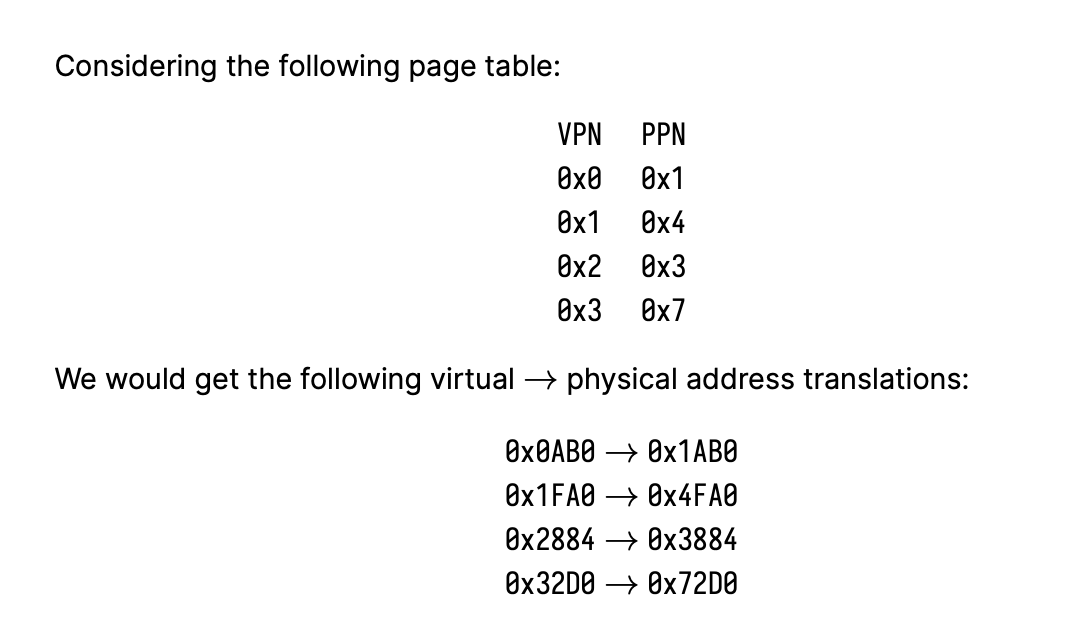
\includegraphics[width=0.8\linewidth]{img/image_2023-02-06-15-31-33.png}
    \caption{Simple page table}
\end{figure}

\subsection{Page Tables}

\begin{itemize}
    \item Naive page tables are not scalable. For example, if we have 4GiB $ 2^{32} $ bytes of virtual memory and a 4 kB ($ 2^{12} $ byte) page size size then the address space should be split into $ 2^{20} $ pages. So the page table must have $ 2^{20} $ entries, each of which requires $ 20 $ ( frame number; $ 2^{20} $ frames), a valid bit, a dirty bit, and read/write/execute permission bits -- a total of 25. So the total size of the page table is on the order of $ 2^{22} $ bytes = 4MB (of which we would need one per process)
\end{itemize}

\begin{figure}[H]
    \centering
    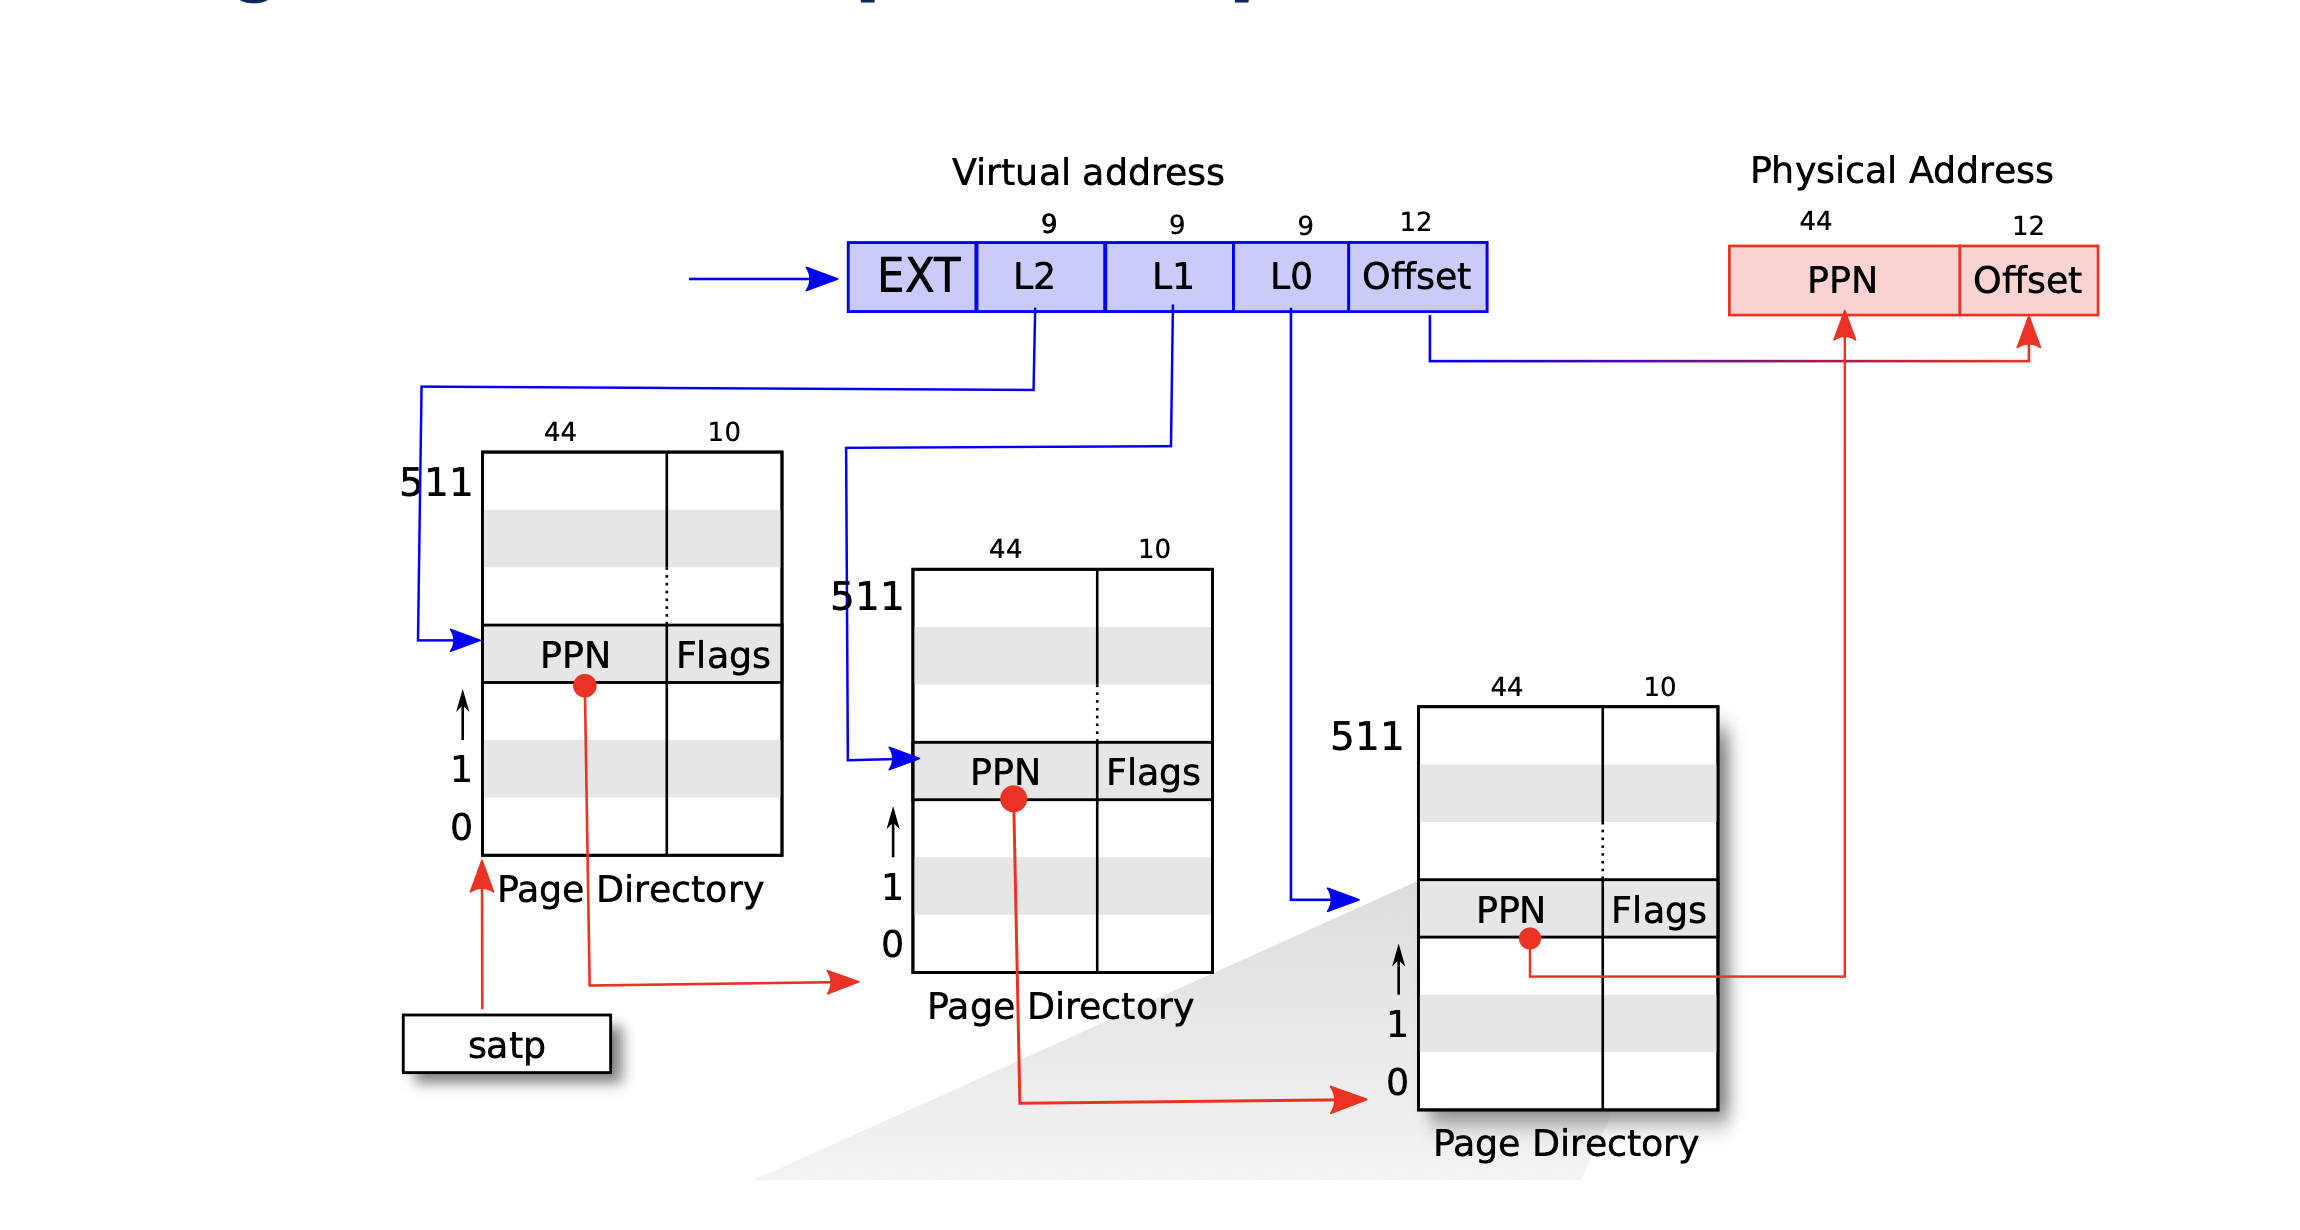
\includegraphics[width=0.8\linewidth]{img/image_2023-02-08-15-15-10.png}
    \caption{Multi-level page tables save storage space for sparse allocations}
\end{figure}

\begin{itemize}
    \item Page allocation usually implemented via a linked list. Allocate page: remove it from the free list; deallocate -- add back to free list.
    \item A page is used for each page table. There are 512 entries of 8 bytes each to make 4096 page tables, so each page table can be treated as an array of 512 page table entires (PTE).
    \item The PTE for L(N) points to the page table for L(N-1) -- so follow these page tables until L0 and that contains the PPN
    \item Each table has it's own root page table (L1).
    \item \texttt{satp} register stores root page table
    \item Think of the highest level page table storing pointers to blocks and then lower level page tables storing pointers to segments within those blocks until we get to the exact memory address we want. It just so happens that these blocks also take on the form of a page table by themselves. 
\end{itemize}

\begin{figure}[H]
    \centering
    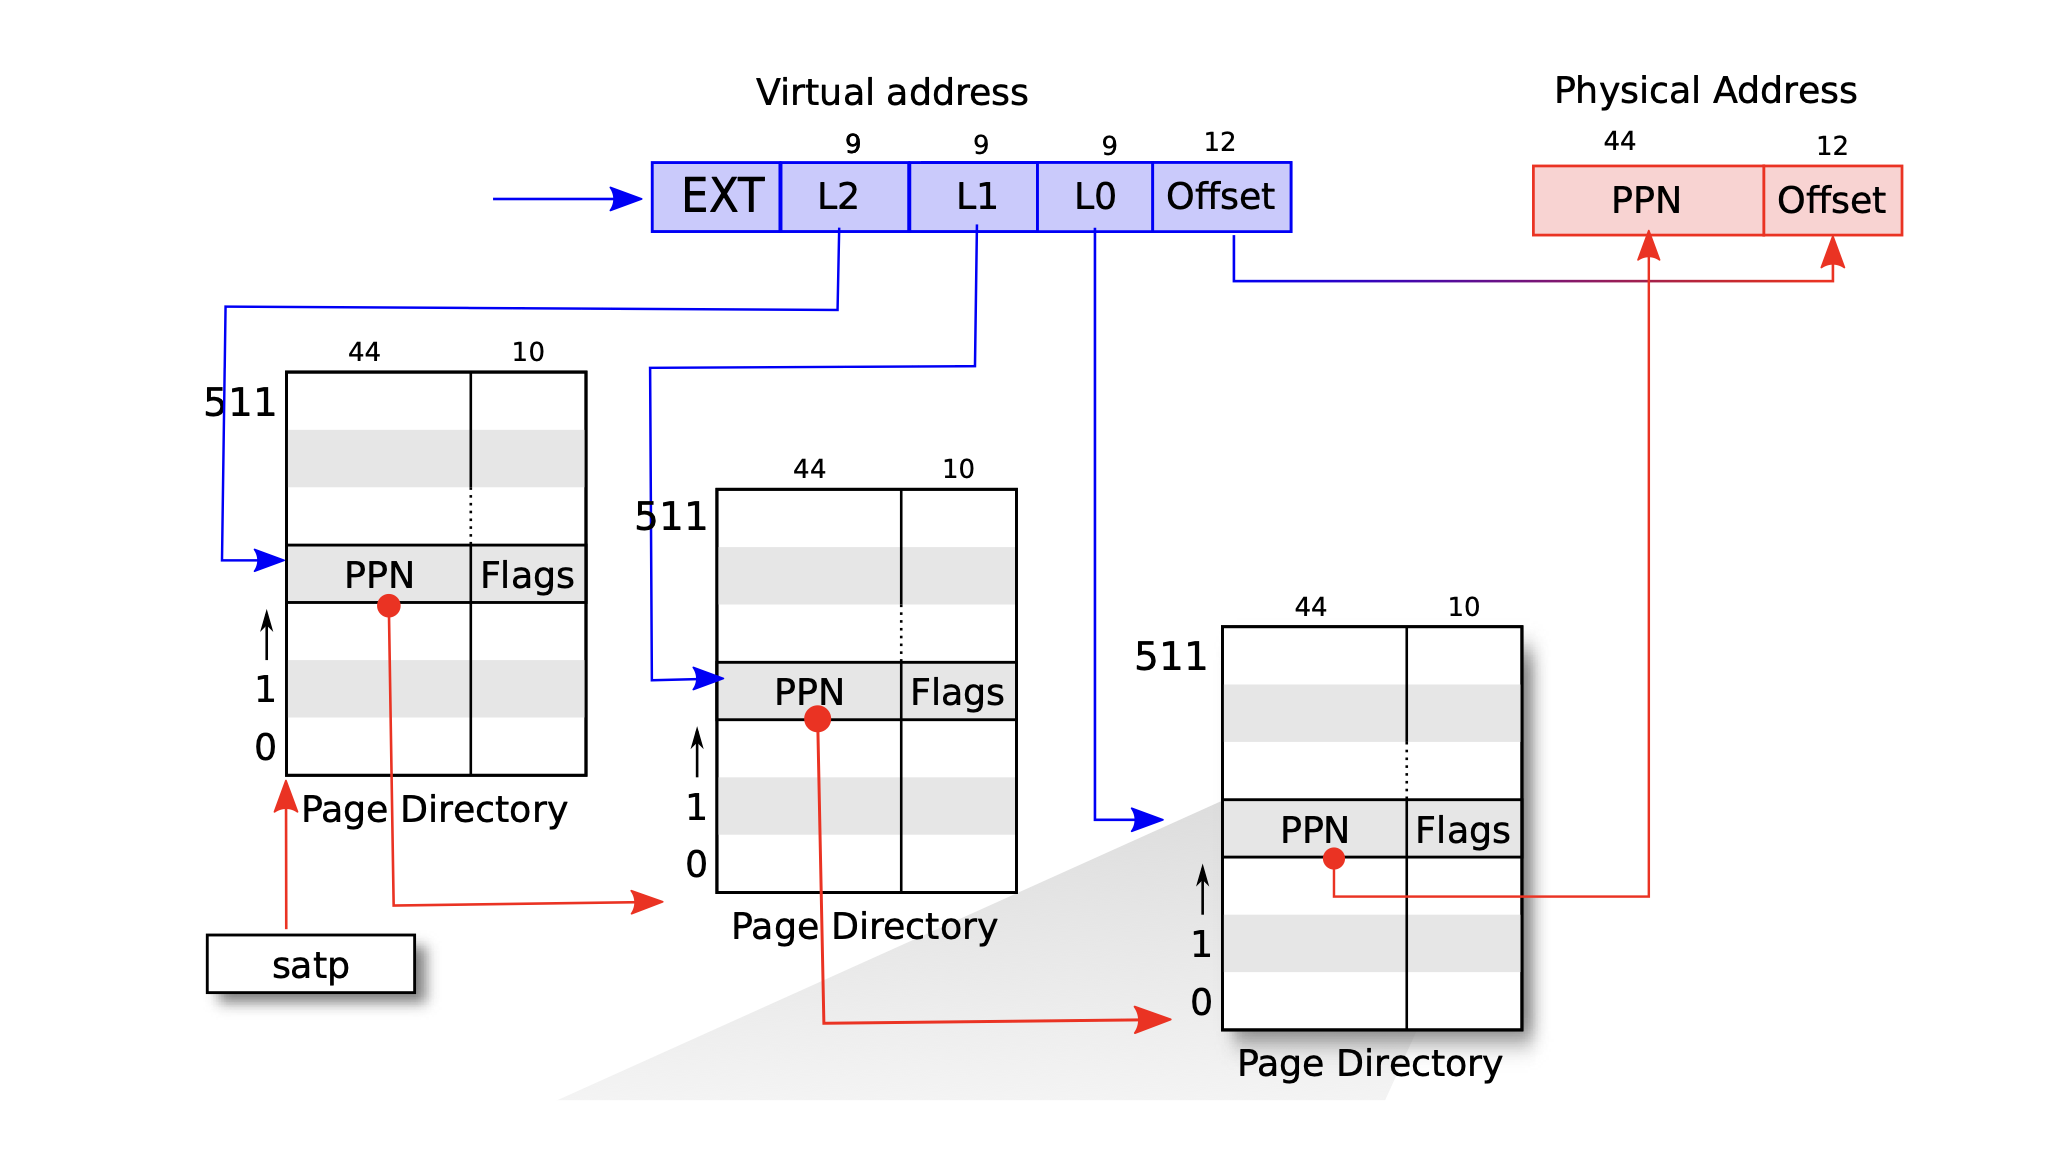
\includegraphics[width=0.8\linewidth]{img/image_2023-02-08-15-50-17.png}
    \caption{Since each page table has 512 entries -- take offset on the address and then split off into 9-bit chunks to get index into each level of the page tables. When we get to the last level simply apply the offset to get the data within the page.}
\end{figure}


\begin{itemize}
    \item Alignment: memory (by usual conventions) eventually line up with zero. For example pages that are 4096-byte have the last 12 bits zeroed.
    \item It would be inconvenient if a page starts at 0x7C00 and has the last byte at 0x88FF; instead in aligned systems a page starts at $ 0x7000 $ and ends at $ 0x7FFF $. \mn{Alternatively addresses that are $ n $-byte aligned are cleanly divisible by $ n $}
\end{itemize}



Following is a snippet of code from class that simulates a page table. It's not a complete implementation but it's a good example of how to use the page table to translate virtual addresses to physical addresses.

\begin{listing}[H]
\begin{minted}{c}
#include <sys/mman.h>
#define PAGE_SIZE 4096

#define LEVELS 3
#define PTE_VALID (1 << 0)

static uint64_t* root_page_table = NULL;
// A wrapper around mmap
static uint64_t* allocate_page_table() {
    void* page = mmap(NULL, PAGE_SIZE, PROT_READ|PROT_WRITE, MAP_ANONYMOUS|MAP_PRIVATE, -1, 0);
    if (page == MAP_FAILED) {
        int err = errno;
        perror("mmap");
        exit(err);
    }
    return page;
}

static void deallocate_page_table(void* page) {
    if (munmap(page, PAGE_SIZE) == -1) {
        int err = errno;
        perror("munmap");
        exit(err);
    }
}
\end{minted}
\end{listing}

\begin{listing}[H]
\begin{minted}{c}
// Looks up a virtual address in the page table and returns the physical address
static uint64_t mmu(uint64_t virtual_address) {
    uint64_t* page_table = root_page_table;
    uint64_t va = (uint64_t) virtual_address;
    for (int i = LEVELS - 1; i >= 0; --i) {
        uint8_t start_bit = 9 * i + 12;
        uint64_t mask = (uint64_t) 0x1FF << start_bit;
        uint16_t index = (mask & va) >> start_bit;

        uint64_t pte = page_table[index];
        if (!(pte & PTE_VALID)) {
            printf("0x%lX: page fault\n", va);
            return 0;
        }

        if (i != 0) {
            page_table = (uint64_t*) ((pte >> 10) << 12);
            continue;
        }

        uint64_t pa = ((pte & ~0x3FF) << 2) | (va & 0xFFF);
        printf("0x%lX: 0x%lX\n", va, pa);
        return pa;
    }
    __builtin_unreachable();
}

// page table entry from physical address
uint64_t pte_from_ppn(uint64_t ppn) {
    uint64_t pte = ppn << 10;
    pte |= PTE_VALID; // set valid bit
    return pte;
}

// page table entry from page number
uint64_t pte_from_page_table(uint64_t* page_table) {
    return pte_from_ppn(((uint64_t) page_table) >> 12);
}
\end{minted}
\end{listing}


\begin{listing}[H]
\begin{minted}{c}
int main() {
    assert(sysconf(_SC_PAGE_SIZE) == PAGE_SIZE);
    uint64_t* l2_page_table_1 = allocate_page_table();
    uint64_t* l1_page_table_1 = allocate_page_table();
    uint64_t* l0_page_table_1 = allocate_page_table();
    uint64_t* l0_page_table_2 = allocate_page_table();
    root_page_table = l2_page_table_1; // global var to set root
    // manually set values at 0xabcdef to something valid
    l2_page_table_1[0] = pte_from_page_table(l1_page_table_1);
    l1_page_table_1[5] = pte_from_page_table(l0_page_table_1);
    // offset for 0xabcdef
    l1_page_table_1[13] = pte_from_page_table(l0_page_table_2);
    l0_page_table_1[188] = pte_from_ppn(0xCAFE);
    // set page table entry to physical address 0xFACE
    l0_page_table_1[188] = pte_from_ppn(0xFACE);
    mmu(0xABCDEF); // [L2: 0][L1: 5][L0: 188] -> 0xCAFEDF
    mmu(0x1ABCDEF); // -> OxCAFEDF
    // two virtual addresses point to the same physical address here.
    // this is how shared memory would be implemented
    deallocate_page_table(root_page_table);
    root_page_table = NULL;
    return 0;
}
\end{minted}
\end{listing}




\begin{listing}[H]
\begin{minted}{c}
int main() {
    assert(sysconf(_SC_PAGE_SIZE) == PAGE_SIZE);
    uint64_t* l2_page_table_1 = allocate_page_table();
    uint64_t* l1_page_table_1 = allocate_page_table();
    uint64_t* l0_page_table_1 = allocate_page_table();
    uint64_t* l0_page_table_2 = allocate_page_table();
    root_page_table = l2_page_table_1; // global var to set root
    // manually set values at 0xabcdef to something valid
    l2_page_table_1[0] = pte_from_page_table(l1_page_table_1);
    l1_page_table_1[5] = pte_from_page_table(l0_page_table_1);
    // offset for 0xabcdef
    l1_page_table_1[13] = pte_from_page_table(l0_page_table_2);
    l0_page_table_1[188] = pte_from_ppn(0xCAFE);
    l0_page_table_1[188] = pte_from_ppn(0xFACE);
    mmu(0xABCDEF); // [L2: 0][L1: 5][L0: 188] -> 0xCAFEDF
    mmu(0x1ABC007); // translates -> 0xFACE007
    deallocate_page_table(root_page_table);
    root_page_table = NULL;
    return 0;
}
\end{minted}
\end{listing}

\begin{itemize}
    \item Let's assume our program uses 512 pages. What's the min and max number of page tables we need? (with a 3-level paging system)
        \begin{itemize}
            \item Min: 3 page tables total; L2 -> L1 -> 512 entries in L0
            \item Max: 1 entry per L1, L0 so 512 tables each, and then 1 table (can only have 1 table for the entry point) in L0 and then -> so 512 * 2 + 1 = 1025 pages tables.
        \end{itemize}
    \item Example: how many levels do we need? 32 bit virtual address space ,page size of 4096, PTE size of 4 bytes. Each page table should fit in a single page. 
        \begin{itemize}
            \item Number of PTEs: $ \log_2(\text{\# PTEs per page}) $ is the number of bits to index a page table
            \item $ \text{number of levels} = \frac{\text{virtual - offset}}{\text{index}} = \frac{32-12}{10} 2$ 
        \end{itemize}
    \item Page tables for every memory access is slow: solution is to use caching
    \item Programs tend to have a lot of memory access patterns and only use a few pages at a time. TLB\mn{Translation Lookaside Buffer} works as cache for virtual address to physical address translation

\end{itemize}

\subsection{Threads}


\begin{itemize}
    \item Threads share memory and enable concurrency within the same process
    \item \texttt{pthread}!
    \item \texttt{join} is the thread equivalent of \texttt{wait}
    \item \texttt{pthread\_detach} release their resources when they terminate. Otherwise (by default) they are joinable and must be joined before resources are released.

\end{itemize}

\subsubsection{Threads Implementation}

\begin{itemize}
    \item Kernels can be implemented in the user or at the kernel level.
    \item User level usually involves fast switching at the user level. These are fast to create, but if one thread blocks it will block the entire process.
    \item Kernel level threads can deal with these blocking threads, but are slower since they require syscalls.
    \item User level threads can be desirable because they can be made to only depend on the c standard library, which is portable
    \item Many-to-one threads map multiple user threads to one kernel thread
    \item One-to-one threads map one user thread to one kernel thread. \texttt{pthread} does this.
    \item Many-to-many is a hybrid approach. This leads to a complicated implementation.
    \item Threads complicate the kernel. For example, how should \texttt{fork} work with a process that has multiple threads? Do we just copy all threads over? Linux will only copy the thread that called fork into a new process and an option at \texttt{pthread\_atfork} which can be used to control the behaviour.
    \item What about signals? On linux this will just be any random thread within that process.
    \item Instead of many-to-many a common technique is to use a thread pool. This creates a set number of threads and a queue of tasks.
    \item Cooperative scheduling: threads must call \texttt{yield}. Pre-emptive scheduling can be implemented by forcing threads to call \texttt{yield}.
\end{itemize}





\subsubsection{Useful tools}

\begin{itemize}
    \item \texttt{tailq} (\texttt{sys/queue.h}) is a header that has a bunch of macros for working on singly and doubly linked lists, queues, and circular queues.
        \begin{itemize}
            \item i.e. \texttt{TAILQ\_ENTRY} is a macro that defines the pointer relations for a doubly linked tail queue
            \item \texttt{TAILQ\_FOREACH} is a macro that iterates over a doubly linked tail queue
            \item \texttt{TAILQ\_INSERT\_SAFE} is a macro that inserts an element into a doubly linked tail queue at the tail
            \item \texttt{TAILQ\_REMOVE} is a macro that removes an element from a doubly linked tail queue
        \end{itemize}
    \item \texttt{ucontext} (\texttt{ucontext.h}) is a header that largely wraps around \texttt{ucontext\_t} which holds the context for a user thread of execution, i.e. stack, saved register, and blocked signals.
    \begin{itemize}
        \item Useful methods include \texttt{getcontext}, \texttt{setcontext}, \texttt{makecontext}, and \texttt{swapcontext}
    \end{itemize}
\end{itemize}


\begin{listing}[H]
\begin{minted}{c}
#include <errno.h> // errno
#include <stddef.h> // NULL
#include <stdio.h> // perror
#include <stdlib.h> // exit
#include <sys/mman.h> // mmap, munmap
#include <sys/signal.h> // SIGSTKSZ
#include <ucontext.h> // getcontext, makecontext, setcontext, swapcontext
#include <valgrind/valgrind.h> // VALGRIND_STACK_REGISTER

static void die(const char* message) {
    int err = errno;
    perror(message);
    exit(err);
}

static char* new_stack(void) {
    char* stack = mmap(
        NULL,
        SIGSTKSZ, // canonical size for signal stack
        PROT_READ | PROT_WRITE | PROT_EXEC,
        MAP_ANONYMOUS | MAP_PRIVATE,
        -1,
        0
    );
    if (stack == MAP_FAILED) {
        die("mmap stack failed");
    }
    VALGRIND_STACK_REGISTER(stack, stack + SIGSTKSZ);
    // tells valgrind this is an unique stack
    return stack;
}

static void delete_stack(char* stack) {
    if (munmap(stack, SIGSTKSZ) == -1) {
        die("munmap stack failed");
    }
}
\end{minted}
\end{listing}

\begin{listing}[H]
\begin{minted}{c}

// the stacks we're going to use in this demo
static ucontext_t t0_ucontext;
static ucontext_t t1_ucontext;
static ucontext_t t2_ucontext;

static char* t1_stack;
static char* t2_stack;

static void t2_run(void) {
    printf("T2 should be done, switch back to T0\n");
    delete_stack(t1_stack);
    setcontext(&t0_ucontext);
}

static void t1_run(void) {
    printf("Hooray!\n");
}


\end{minted}
\end{listing}

\begin{listing}[H]
\begin{minted}{c}

int main(void) {
    /* Creates a new context by copying over the current context, this copies all its
     * registers, and a pointer to its stack (the default kernel allocated one). */
    getcontext(&t0_ucontext);

    /* If we setcontext or swapcontext to t0_context, it'll be as if we just
     * returned from that getcontext call. If you uncomment the line below
     * you'll be in an infinite loop! */
    // setcontext(&t0_ucontext);

    /* Let's create a context that'll execute the run function */
    t1_stack = new_stack();
    getcontext(&t1_ucontext);
    t1_ucontext.uc_stack.ss_sp = t1_stack;
    t1_ucontext.uc_stack.ss_size = SIGSTKSZ;
    /* Uncomment this line to switch to another context when this one ends.
     * By default the process will just exit if a thread makes it to the end
     * of the function.
     */
    // t1_ucontext.uc_link = &t2_ucontext;
    // modifies an initialized context such that when it runs it will
    // call the functions with the arguments provided
    makecontext(
        &t1_ucontext, /* The ucontext to use, it must be initialized with
                       * getcontext */
        t1_run, /* The function to start executing */
        0); /* This is how many arguments we're going to pass to the function */

    t2_stack = new_stack();
    getcontext(&t2_ucontext);
    t2_ucontext.uc_stack.ss_sp = t2_stack;
    t2_ucontext.uc_stack.ss_size = SIGSTKSZ;
    makecontext(&t2_ucontext,  t2_run,  0);

    /* If we just setcontext here when we run T2 after T1 finishes, we'll
     * get into an infinite loop again. */
    // setcontext(&t1_ucontext);
    // exchanges currently active context
    swapcontext(&t0_ucontext, &t1_ucontext);

    printf("Main is back in town\n");
    delete_stack(t2_stack);

    return 0;
}


\end{minted}
\end{listing}

\subsection{Locks}

\begin{itemize}
    \item Concurrent actions accessing the same variable with at least one write can cause a data race
    \item Atomic operations are operations that are guaranteed to be executed in a single step, i.e. non-preemptible.
\end{itemize}

\begin{definition}
    TAC (three-address-code) is an intermediate representation that is used to represent a program in a way where each instruction is atomic -- this is useful for reasoning about data races and can be easier to read than assembly.
    They have the form

    \begin{listing}[H]
    \begin{minted}{text}
    result := operand1 operator operand2
    \end{minted}
    \end{listing}


    For gcc we can see the tac by using the \texttt{-fdump-tree-gimple} or \texttt{fdump-tree-all} flags.
\end{definition}

Let's consider some GIMPLE code produced from a function that increments an integer stored at address \texttt{pcount}

\begin{listing}[H]
\begin{minted}{text}
D.1 = *pcount;
D.2 = D.1 + 1;
*pcount = D.2;
\end{minted}
\end{listing}


\begin{figure}[H]
    \centering
    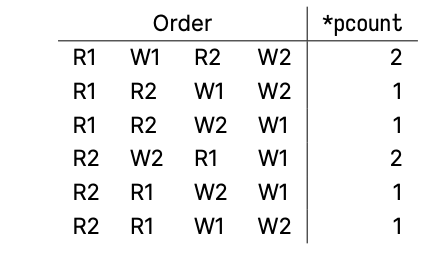
\includegraphics[width=0.8\linewidth]{img/image_2023-03-08-13-21-55.png}
    \caption{Pre-emption possibilities. Let's say we have a producer-consumer model with read/write from two threads. There are many possible orderings of these GIMPLE'd instructions, of which some produce undesirable results}
\end{figure}

\begin{listing}[H]
\begin{minted}{c}
pthread_mutex_t lock = PTHREAD_MUTEX_INITIALIZER;
// or: pthread_mutex_t m; pthread_mutex_init(&m2, NULL)

pthread_mutex_lock(&lock);
// ... critical section: only one thread can access at a time
pthread_mutex_unlock(&lock)
// careful: deadlocks can happen with multiple mutexes.

pthread_mutex_trymutex(&lock); // returns 0 if it was able to lock, otherwise an error code

pthread_mutex_destroy(&lock)
\end{minted}
\end{listing}

How are these implemented?

A naive implementation may look as follows:

\begin{listing}[H]
\begin{minted}{c}
void init(int *l) { *l = 0; }

void lock(int *l) {
while (*l == 1);
*l = 1;}

void unlock(int *l) { *l = 0; }
\end{minted}
\end{listing}

However, this is 1) not safe (both threads can be in the critical section) and not efficient due to the busy wait.


\marginnote{Hardware requirements to implement software locks: atomic load and stores, and instructions execute in order}

Better approaches include Peterson's algorithm and Lamport's bakery algorithm. They have some scalability issues and processors may not execute in order.


Here's another attempt using a magical atomic function: \texttt{compare\_and\_swap} which returns the original value pointed to, and only swaps if the original value equals old and changes it to new.

\begin{listing}[H]
\begin{minted}{c}
void init(int *l) { *l = 0; }
void lock(int *l) { while (compare_and_swap(l, 0, 1)); }
void unlock(int *l) { *l = 0; }
\end{minted}
\end{listing}

\marginnote{\texttt{compare\_and\_swap} is commonly implemented in hardware; on x86 platforms this is implemented using the \texttt{cmpxchg} instruction}

This solves the concurrency issue however it still is not efficient due to the busy wait.

\begin{listing}[H]
\begin{minted}{c}
void lock(int *l) {
while (compare_and_swap(l, 0, 1)) {thread_yield(); }}
\end{minted}
\end{listing}

This is better, but still not ideal. Multiple threads waiting for an event can be awoken when the vent occurs, but only one will win\mn{thundering herd problem}. This cycle will repeat until the herd dies down, but not without causing many freezes along the way. Some sort of order must be placed on the herd -- maybe a FIFO queue?


\begin{listing}[H]
\begin{minted}{c}
void lock(int *l) {
while (compare_and_swap(l, 0, 1)) {
    // add myself to the lock wait queue
    thread_sleep(); }}
void unlock(int *l) { *l = 0;
if (/* threads in wait queue */) {
    // wake up one thread
}}
\end{minted}
\end{listing}

However this suffers from two issues: 1) lost wakeup and 2) wrong thread getting the lock

Consider T1, T2 with T2 holding the lock; what if the context gets switched to T2 before T1 is able to successfully add itself to the wait queue? Then T1 will never get woken up since when T2 unlocks T1 will not be in the wait queue.

Let's consider another scenario: we have three threads T1, T2, and T3, and T2 is holding the lock with T3 in T1 in queue to lock the lock (with T3 before T1). 
T2 may try to wake up the lock, but if the OS swaps to T1 before T2 can wake up T3, then T1 will acquire the lock before T3 does; T1 stole the lock from T3.


A lock-guard pair can be used to fix these problems


\begin{figure}[H]
    \centering
    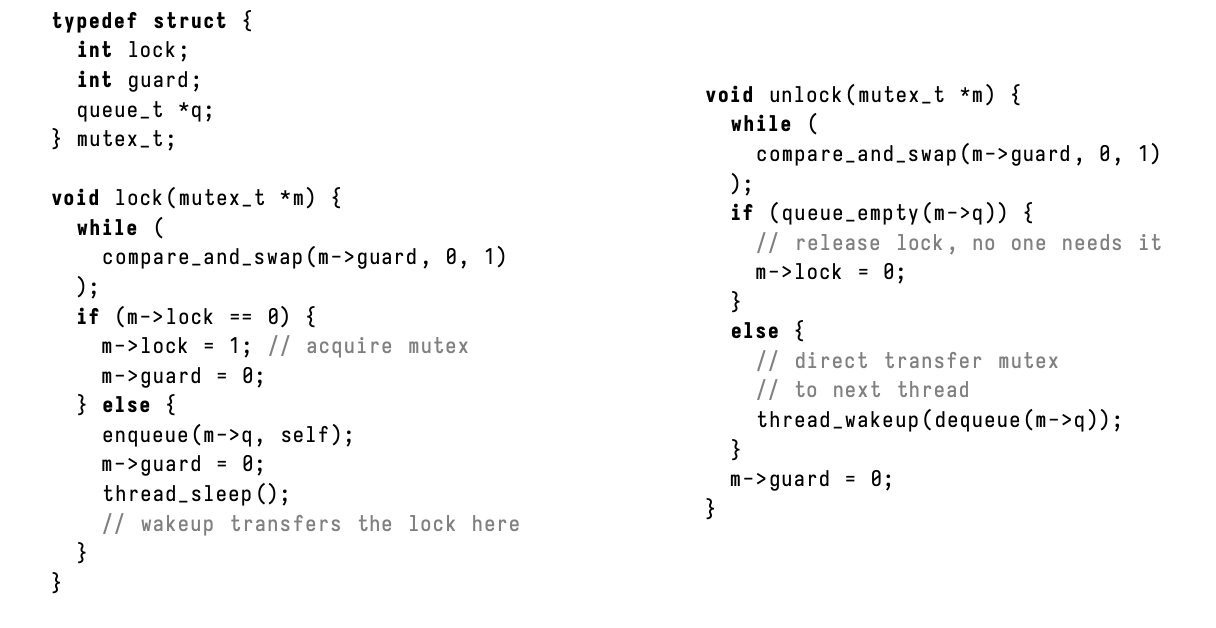
\includegraphics[width=0.8\linewidth]{img/image_2023-03-08-13-52-58.png}
    \caption{A lock-guard pair can be used to make the \texttt{lock} and \texttt{unlock} functions atomic themselves to avoid ugly synchronization issues like those mentioned above}
\end{figure}


However, this does not solve the data race problem: what if a thread gets interrupted right before \texttt{thread\_sleep} (but after being added to the wait queue). So a \texttt{thread\_wakeup} may try to wakeup a thread that isn't sleeping yet.
 A solution may be to poll \texttt{thread\_wakeup}, but this falls back into the busy waiting problem we had before.

A data race is when two concurrent actions access the same variable and at least one of them is a write; we can have as many readers as we want.

Read-write locks (\texttt{pthread\_rwlock\_t} \& co.) are designed to capture this behaviour; multiple threads can hold a read lock (\texttt{pthread\_rwlock\_rdlock}) but only one thread can hold a write lock (\texttt{pthread\_rwlock\_wrlock}) and will wait until current readers are done.

\begin{figure}[H]
    \centering
    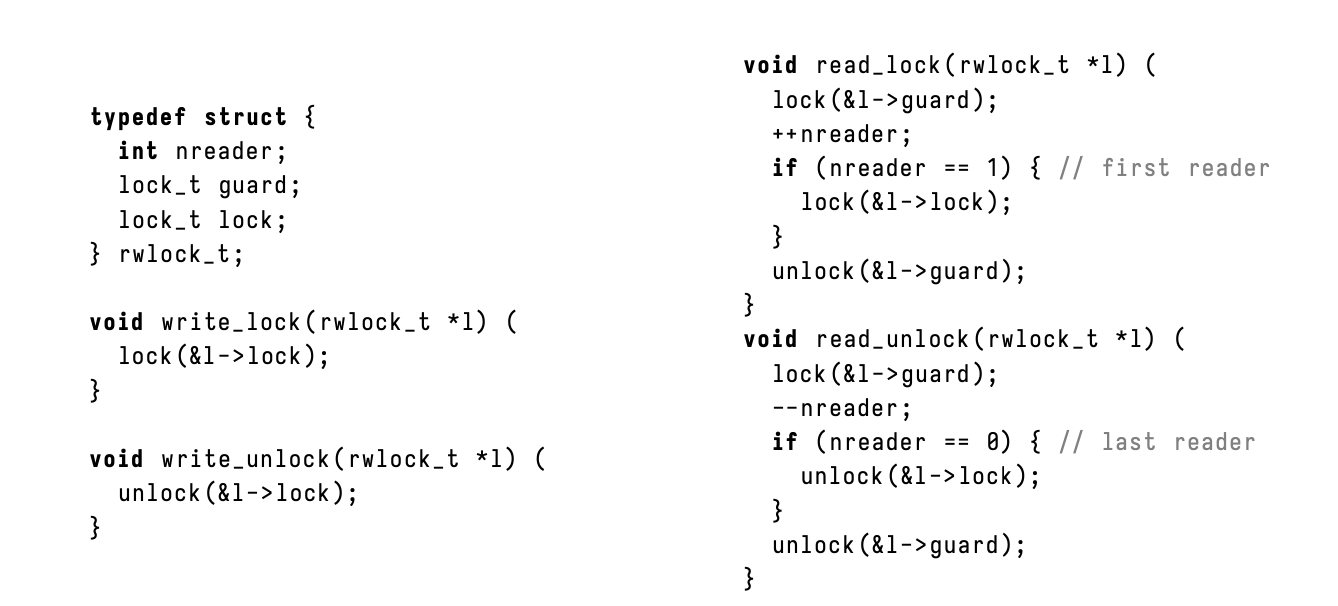
\includegraphics[width=0.8\linewidth]{img/image_2023-03-08-14-02-08.png}
    \caption{rwlock impl}
\end{figure}



\subsection{Semaphores}

Locks (mutexes) enforce \textit{mutual exclusion}, but not necessarily ordering.
But how can we ensure an ordering between two threads?
For example, how can we make one thread always print first?

\begin{definition}
    \textbf{Semaphores} have a value\mn{Usually an integer $ \ge 0 $} that is shared between threads and provide two operations: \texttt{wait} (atomic decrement, blocking) and \texttt{post} (atomic increment).
    Initial \texttt{value} can be set to whatever.
\end{definition}

\begin{figure}[H]
    \centering
    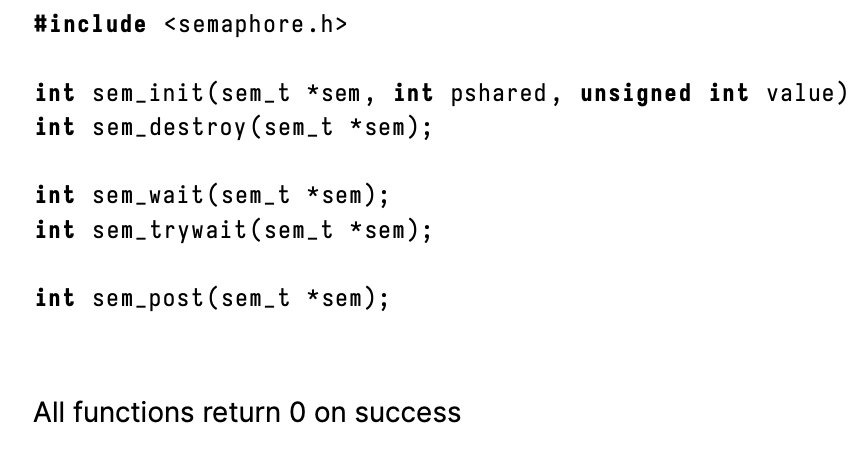
\includegraphics[width=0.8\linewidth]{img/image_2023-03-08-14-08-18.png}
    \caption{Semaphore methods. \texttt{pshared} can be set to 1 for IPC (needs to live in shared mem for IPC)}
\end{figure}




\begin{figure}[H]
    \centering
    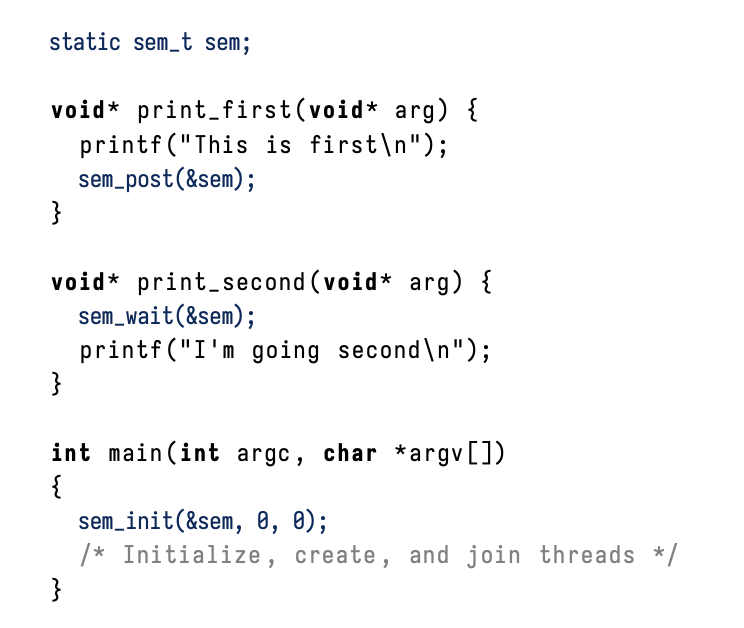
\includegraphics[width=0.8\linewidth]{img/image_2023-03-08-14-09-35.png}
    \caption{A snippet that uses semaphores as signals to \texttt{print\_first} first and \texttt{print\_second} second}
\end{figure}


\marginnote{
    A semaphore is really a generalized mutex; we can consider a mutex as a semaphore with a value of 1.
}

Let's consider the \textit{producer-consumer} problem:

\begin{figure}[H]
    \centering
    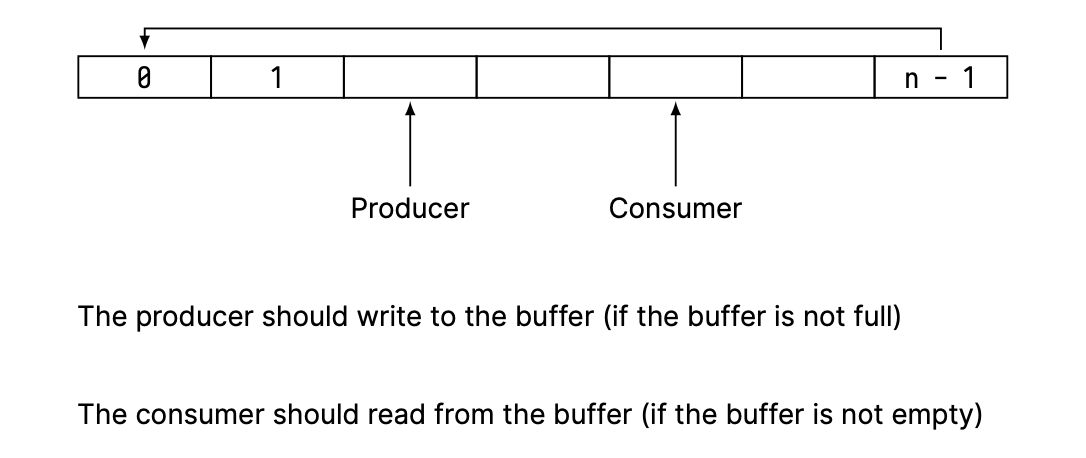
\includegraphics[width=0.8\linewidth]{img/image_2023-03-08-14-11-55.png}
    \caption{All consumers share index $ i_c $, and all producers share index $ i_p $ }
\end{figure}


We can ensure producers never overwrite filled slots by using a semaphore to track the number of empty slots;

\begin{figure}[H]
    \centering
    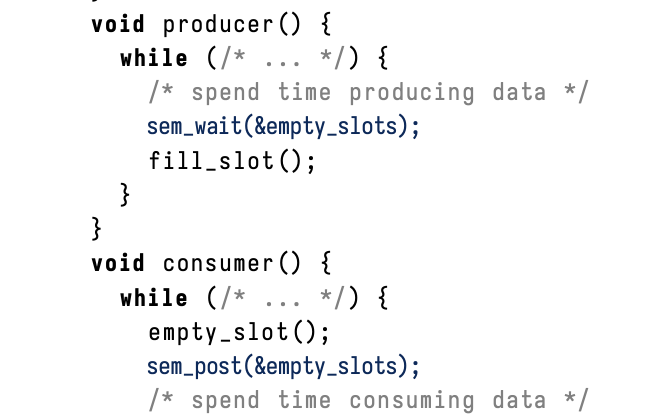
\includegraphics[width=0.8\linewidth]{img/image_2023-03-08-14-14-32.png}
    \caption{Consumer \texttt{post}-s to the empty slots semaphore when done and producer \texttt{wait}-s on the empty slots semaphore before writing}
\end{figure}

A similar semaphore can be used to track the number of filled slots such that consumers never read empty slots;

\begin{figure}[H]
    \centering
    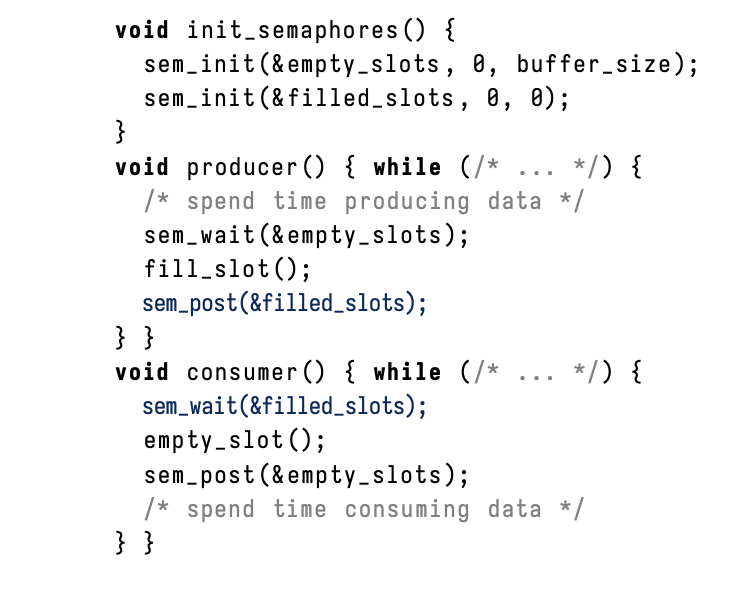
\includegraphics[width=0.8\linewidth]{img/image_2023-03-08-14-15-49.png}
    \caption{Two semaphores ensure proper order}
\end{figure}


\begin{figure}[H]
    \centering
    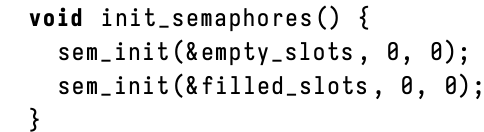
\includegraphics[width=0.8\linewidth]{img/image_2023-03-08-14-32-50.png}
    \caption{Note: Initializing both semaphores to 0 will cause the program to hang because none of the producers will be able to produce anything and then the program just gets stuck}
\end{figure}

\subsection{Locking}

Languages offer support for locking and syntactic sugar. For example, java offers the \texttt{synchronized} keyword:

\begin{figure}[H]
    \centering
    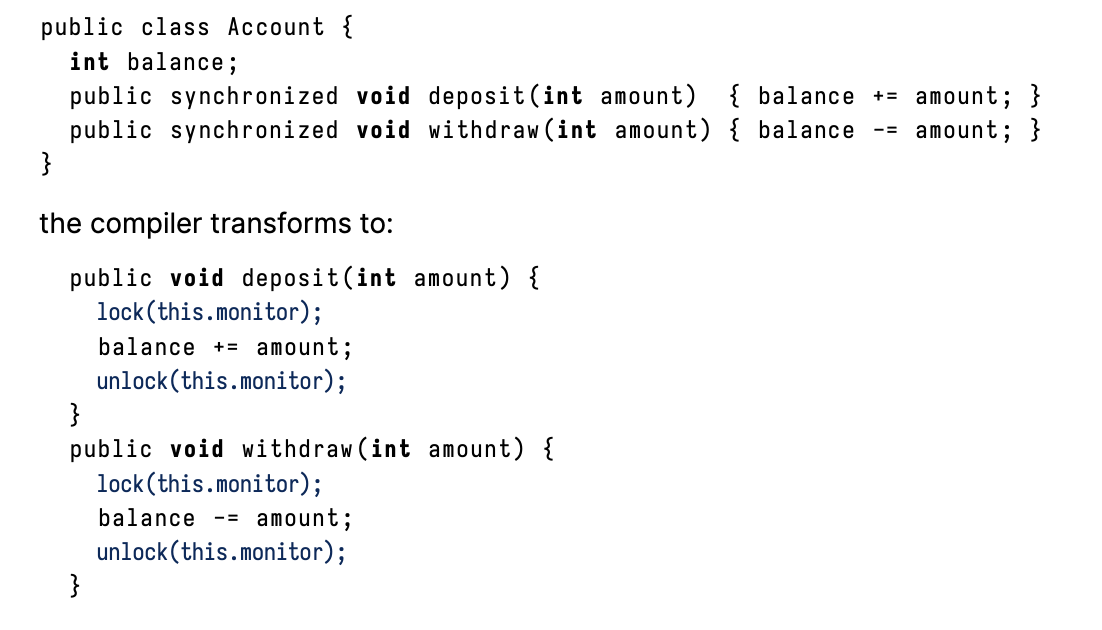
\includegraphics[width=0.8\linewidth]{img/image_2023-03-08-14-37-02.png}
\end{figure}

Another abstraction on top of these synchronization primitives are \textit{condition variables} which enable inter-thread signaling.
\begin{figure}[H]
    \centering
    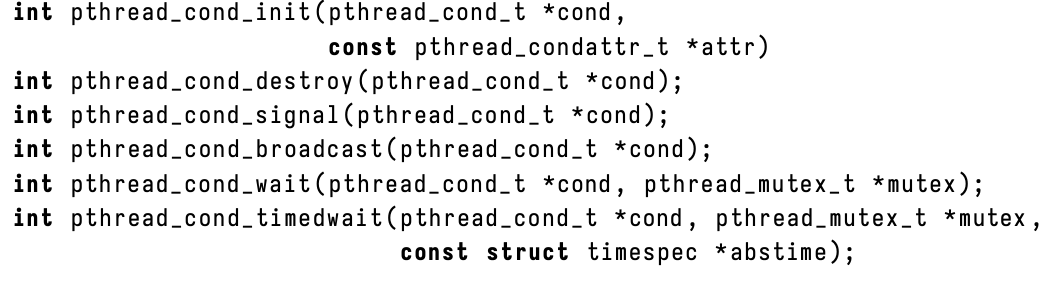
\includegraphics[width=0.8\linewidth]{img/image_2023-03-08-14-38-47.png}
\end{figure}

These condition variables must be paired with a mutex\mn{One mutex can protect multiple condition variables}; any calls to wait must already hold it (but signal/broadcast may not).
The mutex is used to protect the condition variable itself, i.e. to prevent undesirable state changes in the condition variable due to synchronization problems.

\begin{figure}[H]
    \centering
    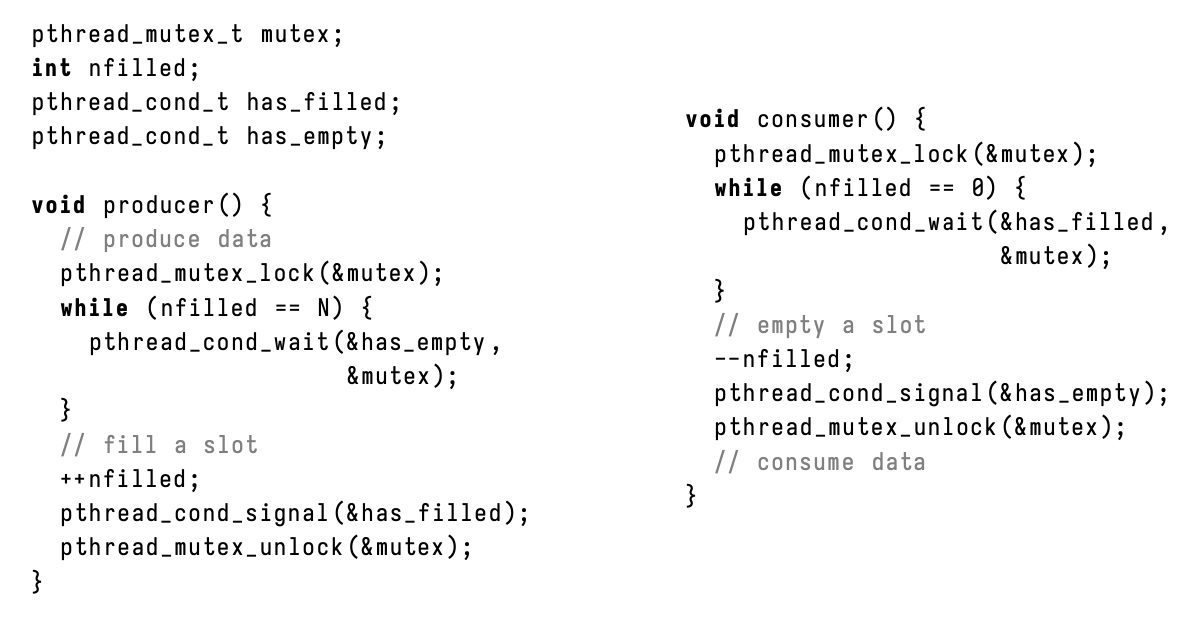
\includegraphics[width=0.8\linewidth]{img/image_2023-03-08-14-44-09.png}
    \caption{Condition variables offer a more elegant solution to the producer-consumer problem}
\end{figure}



\begin{figure}[H]
    \centering
    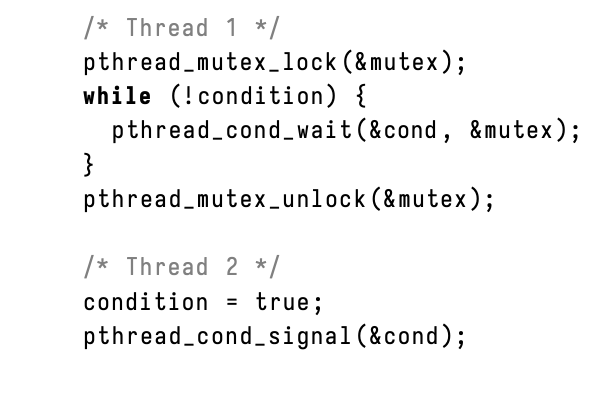
\includegraphics[width=0.8\linewidth]{img/image_2023-03-08-14-45-57.png}
    \caption{Example: This piece of code is a problem because there is no mutex on the \texttt{condition=true} line which can cause the \texttt{while} to produce undesired behaviour. Consider the case where if thread 1 executes first and then it gets swapped away right at the first $ !condition $. Then in thread 2 the condition is to be set to true and the signal is sent without anything happening -- which causes the \texttt{pthread\_cond\_wait} to hang. This can be fixed by locking and unlocking around the \texttt{condition=true} and \texttt{signal} lines.}
\end{figure}


\begin{figure}[H]
    \centering
    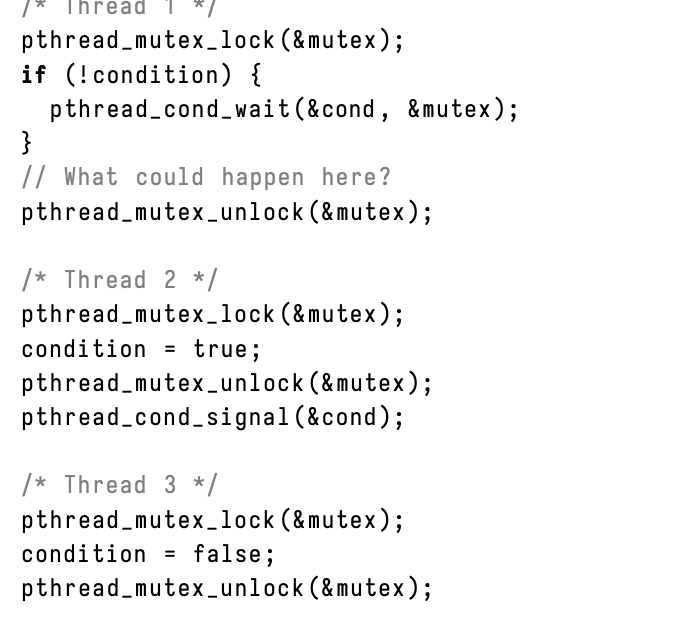
\includegraphics[width=0.8\linewidth]{img/image_2023-03-08-14-53-14.png}
    \caption{Can we change the \texttt{while} to an \texttt{if}?}
\end{figure}

What if we want to avoid polling by changing the \texttt{while} to an \texttt{if}? A problem may occur here.

\begin{enumerate}
    \item T1 goes first w/ initial condition false, cond 0, mutex 0
    \item T1 locks mutex, so no races to worry currently
    \item Put ourselves into condition variable's wait queue, and then unlock mutex
    \item Thread 2 runs: locks mutex, sets condition to true, unlocks, and signals
    \item Thread 1 can now wake up, condition is true, and then it can continue working
    \item But Thread 3 can also wake up, set condition to true, and then transfer context to T2 which signals to T1.
        \begin{itemize}
            \item Now T1 wakes up and by the time it gets to the \texttt{unlock} \texttt{condition} is false, which is a problem (since we wanted \texttt{condition} to be true T1 unlocks (as per the if statement))
        \end{itemize}
\end{enumerate}






Semaphores can be thought of as a special case of condition variables: though one can be implemented with the other it can get messy. Complex conditions are generally implemented with condition variables to keep things clean.

\begin{definition}
    \textbf{Locking Granularity} is the extent to which a lock is held. Too many locks or locks covering large swathes of the program can slow down your program, so it's important to design critical sections carefully. 
\end{definition}


\subsection{Deadlocks}
Deadlocks are a problem. Conditions for deadlocks include:

\begin{itemize}
    \item mutual exclusion
    \item hold and wait (have a lock and try to acquire another)
    \item No preemption (can't take simple locks away)
    \item circular wait (waiting for a lock held by another process)
\end{itemize}

\begin{figure}[H]
    \centering
    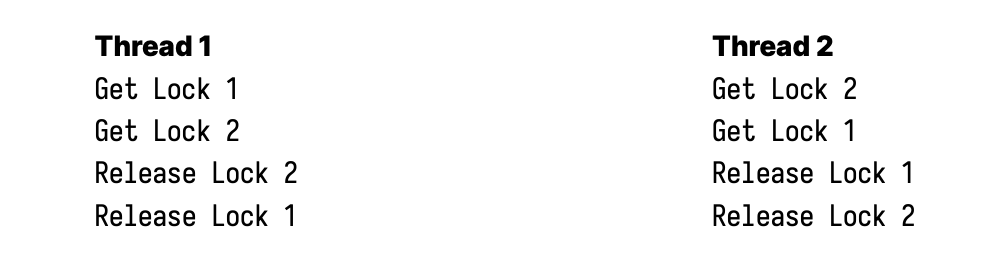
\includegraphics[width=0.8\linewidth]{img/image_2023-03-08-14-58-38.png}
    \caption{This can deadlock depending on the order of the processes trying to get the locks!}
\end{figure}


\begin{figure}[H]
    \centering
    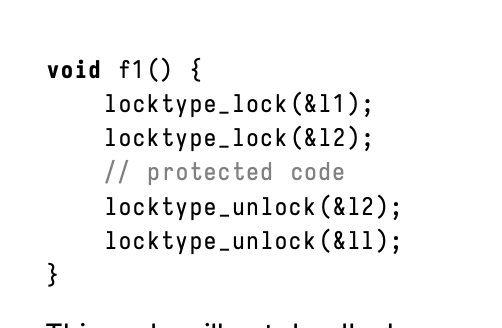
\includegraphics[width=0.8\linewidth]{img/image_2023-03-08-14-59-08.png}
    \caption{Enforcing order is one way to prevent deadlocks}
\end{figure}


\begin{figure}[H]
    \centering
    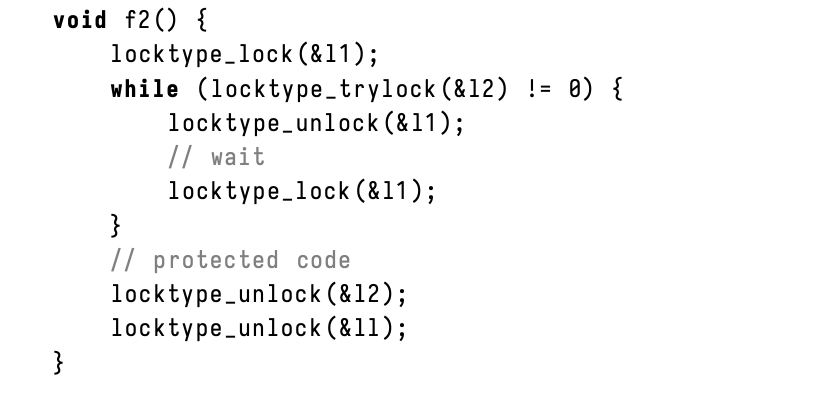
\includegraphics[width=0.8\linewidth]{img/image_2023-03-08-14-59-23.png}
    \caption{Alternatively, \texttt{try\_lock} can be used to self-pre-empt in order to avoid deadlocking}
\end{figure}


See the \texttt{banksim.c} example


// TODO: take exercpts from banksim


\begin{blockquote}
    Note from review session: \texttt{fork} from a \texttt{pthread} will fork with just the calling thread.
\end{blockquote}









\subsection{File Systems}


\begin{figure}[H]
    \centering
    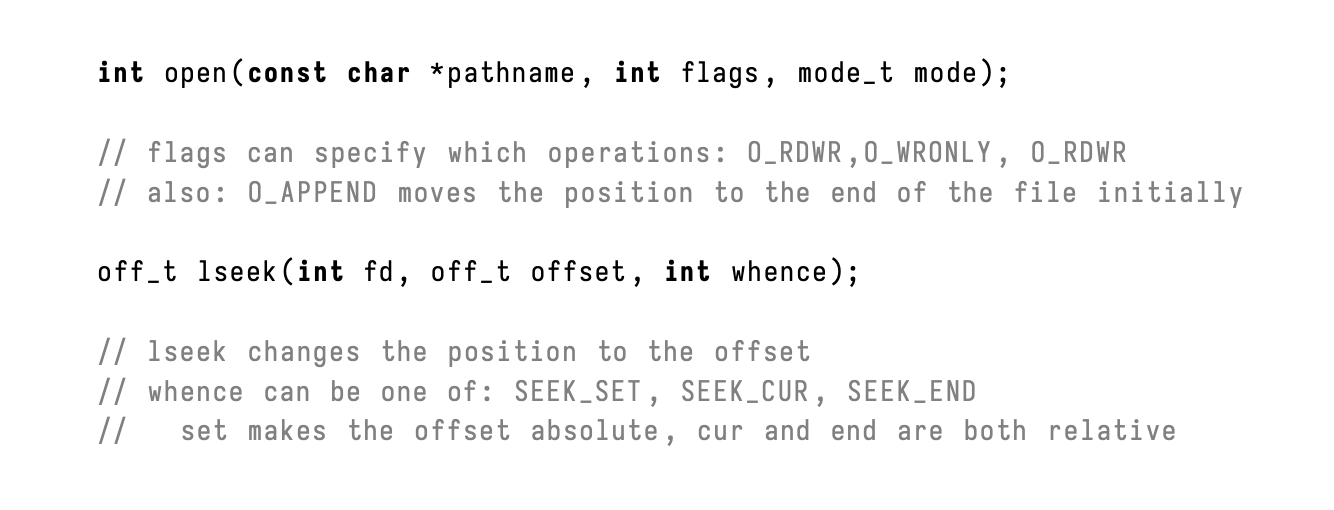
\includegraphics[width=0.8\linewidth]{img/image_2023-03-15-18-18-36.png}
    \caption{Common methods for interacting with the filesystem}
\end{figure}

\begin{figure}[H]
    \centering
    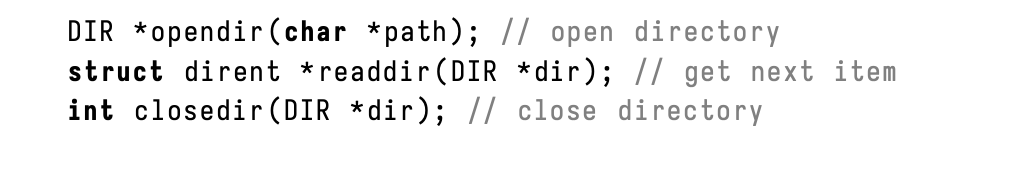
\includegraphics[width=0.8\linewidth]{img/image_2023-03-15-18-18-54.png}
    \caption{Directory methods}
\end{figure}

File tables are stored in the PCB (process control block) and point to the underlying file in the OS.

\begin{figure}[H]
    \centering
    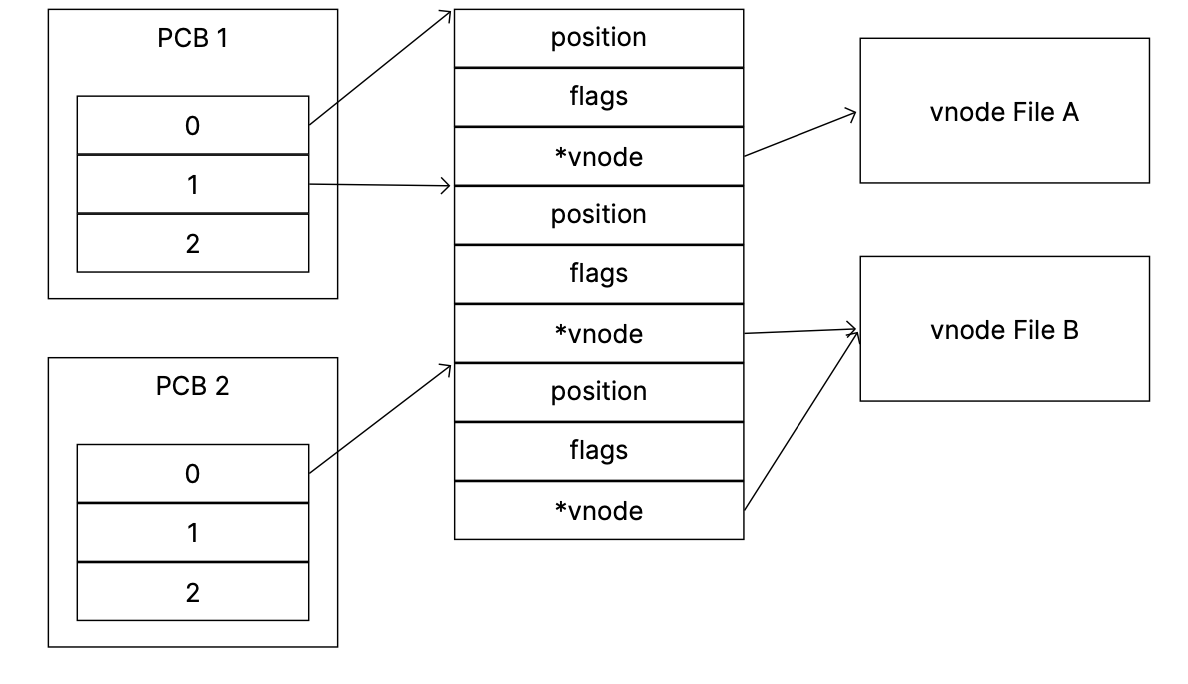
\includegraphics[width=0.8\linewidth]{img/image_2023-03-15-18-19-46.png}
\end{figure}

Each processes has their own file table in its PCB\mn{File descriptors are indexs into that table} and these PCB file table entries then point to a global open file table (GOF) which holds information about the flags and seek position etc. This also houses the vnode\mn{virtual node} which holds information abotu the file (which can be sockets, regular files, mounts, pipes, etc).
This implies that the current position in file is shared between processes and \texttt{seek} operations in one process leads to \texttt{seek} in the other processes. However, opening the same file in processes after a \texttt{fork} creates multiple GOF entries.

\begin{figure}[H]
    \centering
    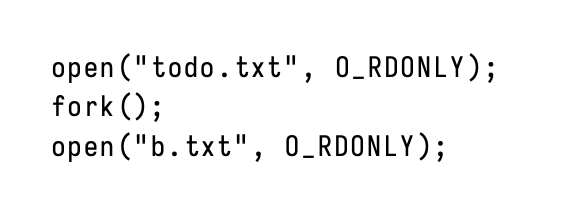
\includegraphics[width=0.8\linewidth]{img/image_2023-03-15-18-30-11.png}
    \caption{For example, this snippet will produce two LOF (Local Open File table) and three GOF entries}
\end{figure}


\begin{figure}[H]
    \centering
    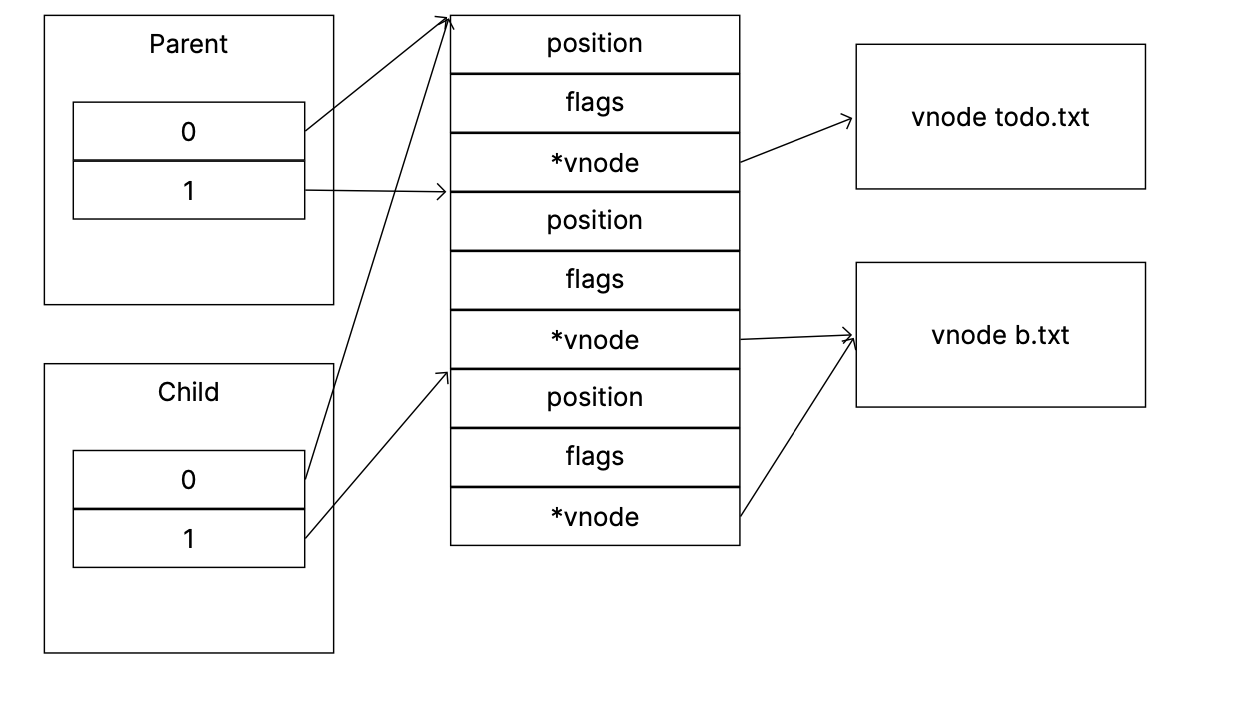
\includegraphics[width=0.8\linewidth]{img/image_2023-03-15-18-31-01.png}
\end{figure}


How are files stored on disk?

\begin{itemize}
    \item Contiguous allocation: Space efficient and with fast random access (block = floor(offset/blocksize)). But cannot be resized easily and fragmentation is a problem.
    \item Linked allocation: Each block has a pointer to the next block. This is more flexible but random access is slower.
    \item FAT (File Allocation Table): The linked list is no longer on-disk but s instead stored on a separate table. The FAT can be held in memory so random access is sped up.
    \item Indexed Allocation: Each block has a pointer to a table of pointers to the next block. However file size is limited by the maximum size of the index block.
\end{itemize}

\begin{example}
    An index block stores pointers to data blocks only. Disk blocks are 8Kib, pointer to a block is 4 bytes. What is the maximum size of a file managed by this index block?

    There are $ \frac{8Kib}{4b} = 2^{11} $ pointers (and addressable blocks needed) so the total number of bytes is $ 2^{11 } * 2 ^{ 13 } = 2^{24} $ = 16Mib



\end{example}





\subsection{inodes}

\begin{figure}[H]
    \centering
    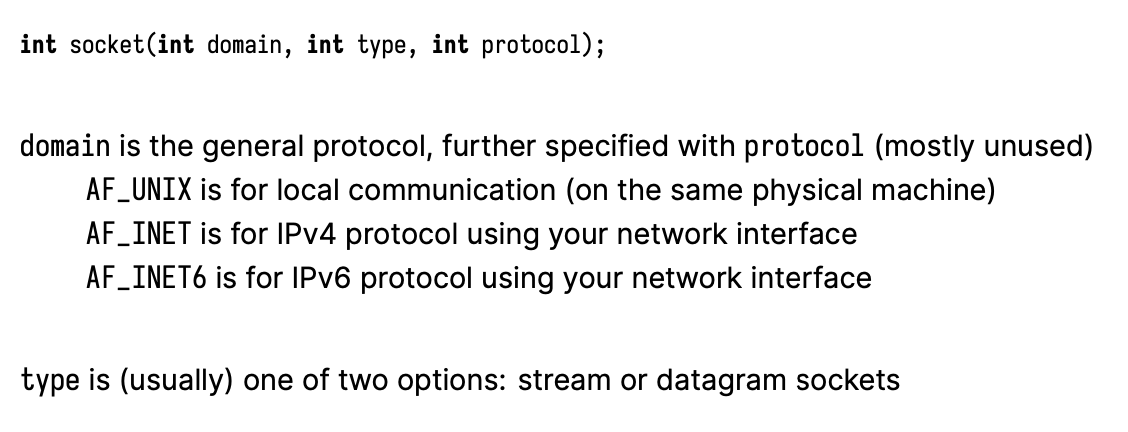
\includegraphics[width=0.8\linewidth]{img/image_2023-03-21-15-09-34.png}
    \caption{\texttt{socket} sets protocol and type of socket}
\end{figure}

\texttt{inodes} describe a file system object. They contain metadata and pointers to block(s)\mn{Small files can just use direct pointers, whereas larger files have additional nodes with pointers to more blocks. Very very small files may live entirely in the inode}

\begin{figure}[H]
    \centering
    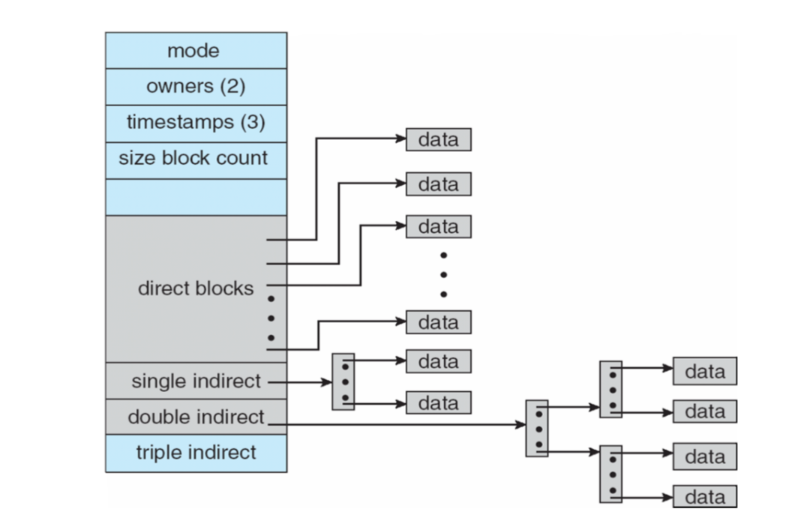
\includegraphics[width=0.8\linewidth]{img/image_2023-03-16-17-48-45.png}
\end{figure}


\begin{figure}[H]
    \centering
    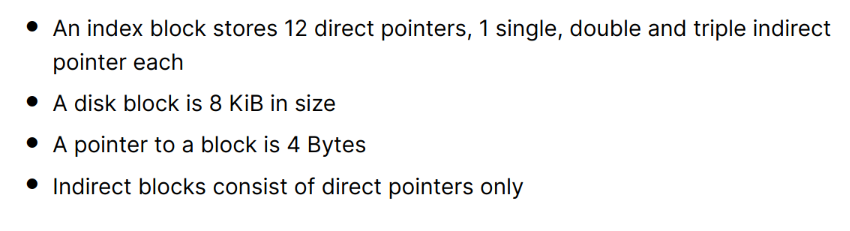
\includegraphics[width=0.8\linewidth]{img/image_2023-03-16-17-49-55.png}
    \caption{\# pointers per indirect table: $2^{13}/2^2 = 2^{11}$. Num of addressable blocks = $ 12 + 2^{11} + (2^{11})^2 + (2^{11})^3 \approx 2^{33} $. Total bytes is $ 2^{33} \cdot  2^{13} = 64 TiB $}
\end{figure}


Hard links\mn{Directory entry} are pointers to one inode. Multiple hard links can point to the same inode, deleting a file only removes a hard link.
Soft links are paths to another file, and are stored as a file. They are not pointers to an inode, but rather a path to another file. Accessing a soft link resolves these links until we reach an inode, an unresolvable soft link leads to an exception.


\subsubsection{Everything is a file}

In UNIX everything is a file\mn{Or some type thereof}. Block devices are files, sockets are files, pipes are files, etc. Directories are files that store filenames and pointers to inodes. 


\begin{figure}[H]
    \centering
    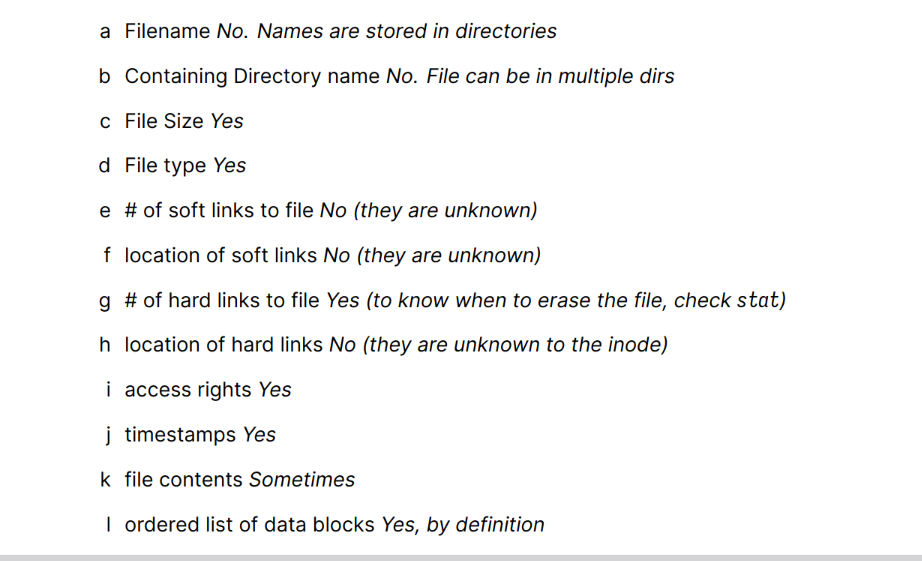
\includegraphics[width=0.8\linewidth]{img/image_2023-03-16-17-59-51.png}
    \caption{Some things that are/are not stored in an inode}
\end{figure}

Note that the inode does not know about the softlinks to it, nor the location of its hard links. However it does store the number of hard links to it so that the kernel can erase the file\mn{use \texttt{stat} to explore this}.

\subsubsection{Caches}

Writing to the disk is slow so file blocks are cached in memory in the filesystem cache\mn{Explore temporal and spatial locality}. A daemon periodically writes changes to the disk\mn{Can manually trigger via \texttt{flush} or \texttt{sync}}.
Deleting a file then involves three steps: 1. removing it's directory entry, releasing the inode to the pool of free inodes, and 3. returning blocks to the pool of free blocks.
Since crashes can happen at any time, UNIX systems are generally built on journaling filesystems, which are filesystems that keep a circular buffer of changes made. This allows for recovery from crashes as well as improving performance by reducing the number of writes to the disk. 






\subsection{Sockets}

Sockets are another way to enable IPC, but over the network (i.e. possibly between different machines).
Use follows a server-client model, where the server sets up sockets via the \texttt{socket, bind, listen,} and \texttt{accept} system calls. The client has \texttt{socket} and \texttt{connect}.
\texttt{socket} creates a socket, \texttt{bind} attaches the socket to some location (file, port, etc), \texttt{listen} to indicate that connections are to be accepted, and \texttt{accept} to accept them. \texttt{connect} connects to an existing socket and enables the socket to send/receive data.
\texttt{UNIX} sockets are for IPC between processes on the same machine, whereas \texttt{AF\_INET} or \texttt{AF\_INET6} is for IPv4 and IPv6 between machines over the network respectively.
Sockets can usually be of two \texttt{type}-s: stream (TCP) and datagram (UDP). TCP is reliable and handshakes and ordered, while UDP is unreliable and unordered.

\begin{itemize}
    \item \texttt{bind} sets socket to an address. Different \texttt{sockaddr} structures are available for different protocols
        \begin{figure}[H]
            \centering
            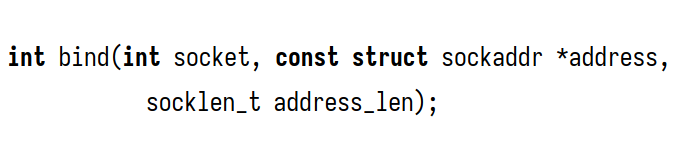
\includegraphics[width=0.8\linewidth]{img/image_2023-03-22-01-01-37.png}
            \label{fig:}
        \end{figure}
    \item \texttt{int listen (int socket, int backlog)} system call sets queue limits for incoming connections

    \item \texttt{int accept(int socket, struct sockaddr* address, socklen\_t* address\_len)} system call accepts a connection on a socket and may block until a connection is made. Returns a new FD that we can write to.
    \item \texttt{int connect(int sockfd, const struct sockaddr* addr, socklen\_t addrlen)} system call connects to a socket. If it succeeds sockfd can be used as a fd.
    \item Instead of \texttt{read} or \texttt{write} there is also \texttt{send} and \texttt{recv} system calls which also have flags as well as \texttt{sendto}/\texttt{recvfrom} which takes an address.
\end{itemize}


\begin{blockquote}
    TODO: sockets example
\end{blockquote}


\subsection{Memory Hierarchy}
\begin{figure}[H]
    \centering
    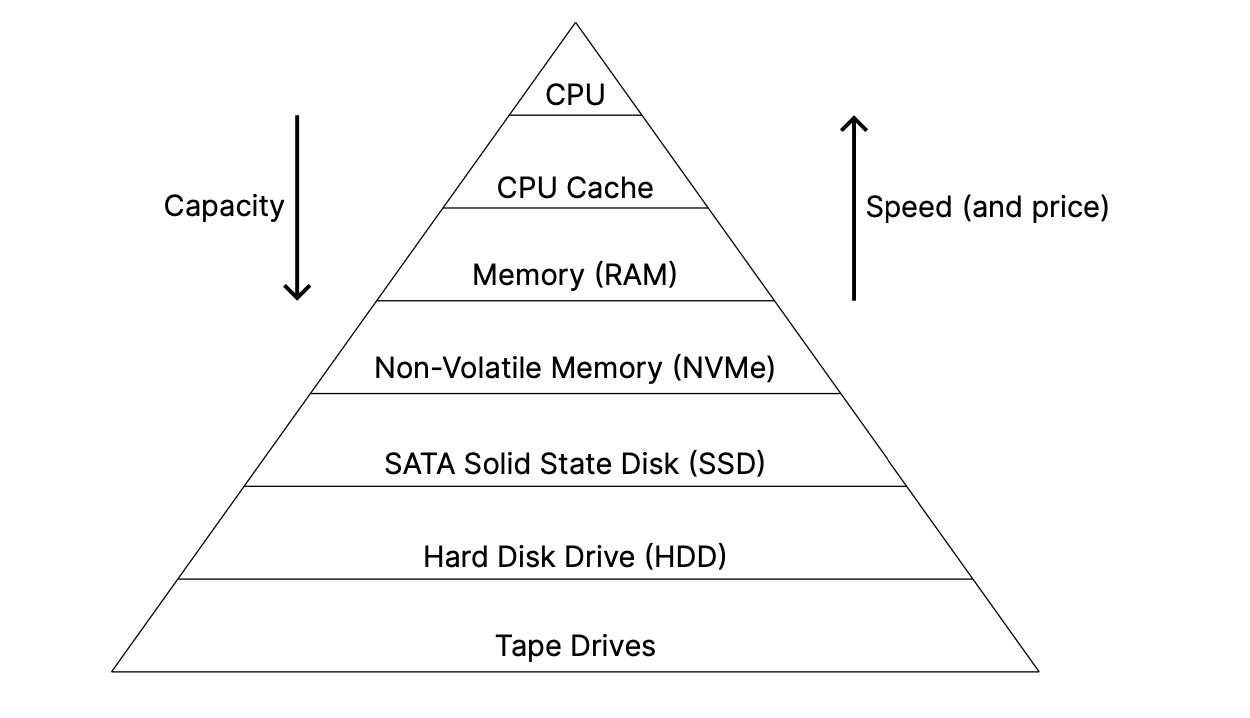
\includegraphics[width=0.8\linewidth]{img/image_2023-03-29-13-48-02.png}
\end{figure}
There is an inversely proportional relationship between computer memory capacity and speed/price, so modern computers use a combination of different memory devices i.e. CPU Cache -> RAM -> SSD -> HDD to store and manage data.
However, we want to abstract this away for the user; each level wants to pretend it has the speed of the level about it and the capacity of the layer below. 
This is done through \textit{paging}: something we've talked about before but will go into further detail now.

Here are some common page replacement policies, or what to do when there is a \textit{page fault}\mn{When a request to the page table is made but the requested page isn't currently in memory}
\begin{enumerate}
    \item Optimal: replace page that won't be used the longest
    \item Random: Replace a random page
    \item FIFO: replace oldest page first
    \item LRU: replace page that hasn't been used for the longest time
\end{enumerate}


\begin{figure}[H]
    \centering
    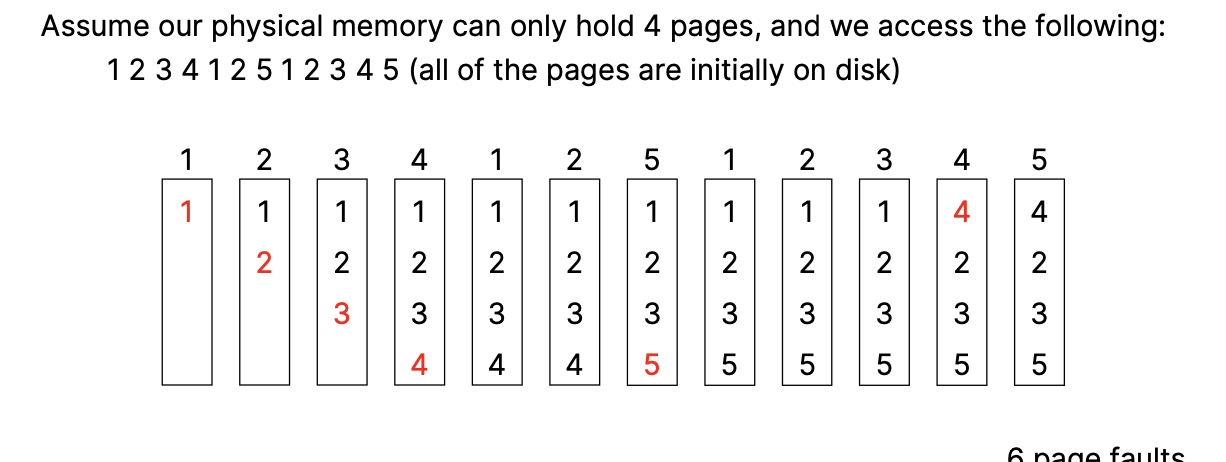
\includegraphics[width=0.8\linewidth]{img/image_2023-03-29-13-49-43.png}
    \caption{Example of using the optimal page replacement policy. Note that 4 gets replaced by 5 since it will get used after 1, 2, 3. Though in this contrived example we know what pages our program will access ahead of time, in practice this is not the case.}
\end{figure}

\begin{figure}[H]
    \centering
    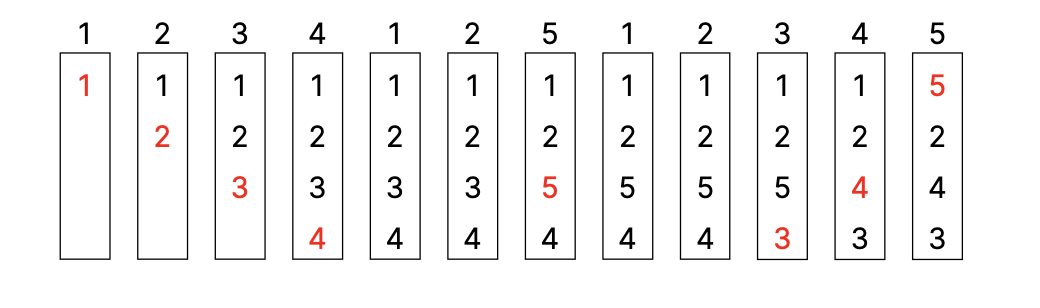
\includegraphics[width=0.8\linewidth]{img/image_2023-03-29-13-53-24.png}
    \caption{A LRU example with FIFO to break ties}
\end{figure}

A downside of using LRU is that it has to search all pages. This can be implemented via a counter or a clock. In software it's also too expensive: you need a doubly linked list of pages and a ton of traversal/manipulation time.
In practice we just use approximate LRU\mn{LRU is just an approximation of optimal anyways}

TLDR:

\begin{itemize}
    \item Optimal isn't realistic
    \item Random works surprisingly well and avoids worst case
    \item FIFO: easy to implement but suffers for Beladay's anomaly\mn{Increasing the number of page frames results in an increase in the number of page faults for certain memory access patterns. FIFO suffers from this but stack-based (LRU) doesn't}
    \item LRU: expensive to implement
\end{itemize}


A more sophisticated page replacement algorithm is the \textit{clock replacement} algorithm

\begin{definition}
    Clock Page Replacement Algorithm:

    \begin{itemize}
        \item Keep a circular list of pages in memory
        \item Use a reference bit for each page in memory
        \item Has a hand pointing to the last element examined
    \end{itemize}

    To insert a new page:
        \begin{itemize}
            \item Check the hand's reference bit: if 0 place page + advance
            \item If 1: set to 0, advance hand, repeat
        \end{itemize}
        Page accesses set the reference bit to 1\mn{And I believe set the hand to the read bit}
\end{definition}

\begin{figure}[H]
    \centering
    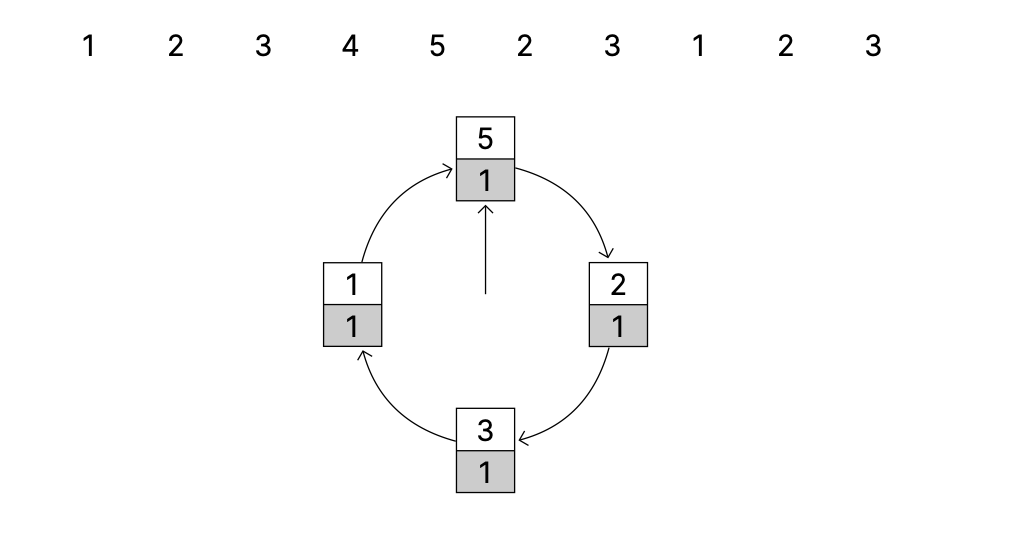
\includegraphics[width=0.8\linewidth]{img/image_2023-03-29-14-00-13.png}
\end{figure}
\marginnote{This is kind of just like using a circular buffer to maintain our page table, but with a pseudo-LRU policy maintained via setting reference bit to 1 on accesses}


\begin{figure}[H]
    \centering
    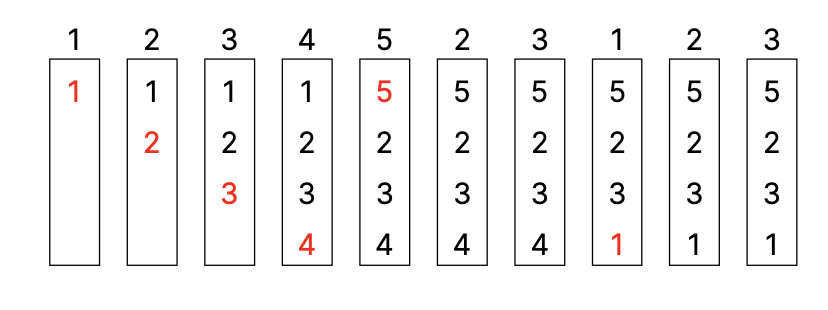
\includegraphics[width=0.8\linewidth]{img/image_2023-03-29-14-00-22.png}
\end{figure}

\subsection{Memory Allocation}

There are two main ways to allocate memory: \textit{static} and \textit{dynamic} allocation. Static allocation is done at compile time, and dynamic allocation is done at runtime.
Static allocation is pretty easy to implement and understand: just give it a fixed size and you're done. However, it can be wasteful or limiting since we don't always know how much memory we'll need at compile time.
We can allocate dynamic memory on the stack or the heap. \texttt{c} largely does stack allocation for you, but the problem is that the scope of stack allocated memory is limited to the scope in which it was allocated.
However, dynamic allocation can pose a problem: since we allocate memory in different sized contiguous blocks, compaction is not possible and every allocation decision is permanent. 
This can leave holes in memory that need to be managed and taken into consideration when allocating memory\marginnote{Note that in $ c $ previous allocations cannot be relocated by the runtime (like Java does, since Java can move the memory around for you)}
Generally speaking there are three cases that lead to fragmentation:

\begin{enumerate}
    \item Different allocation lifetimes
    \item  Different allocation sizes
    \item Inability to relocate previous allocations
\end{enumerate}


Also, there exists two different types of fragmentation: \textit{external} and \textit{internal}. External fragmentation is when different sized blocks are allocated and there isn't enough space between the blocks to allocate. Internal fragmentation occurs when we allocate fixed sized blocks and there is excess space within the blocks.

In our \texttt{malloc} implementations we want to minimize fragmentation\mn{Large applications i.e. chrome will actually ship their own allocators to minimize fragmentation}.
As a guiding heuristic we want to reduce the number of holes between blocks of memory, and if there are holes, we want them to be as large as possible.

Most implementations use a free list: free blocks are chained together with a doubly linked list. Allocation is done by finding a suitable block and removing it from the free list, and deallocation is done by moving the block back to the free list.

There are three general heap allocation strategies best(find smallest block that can satisfy the request), worst (choose largest block), and first fit (choose first fit that can satisfy the request).
From simulations best fit tends to leave very large holes and very small holes, worst it tends to be the worst in terms of storage utilization, and first-fit tends to be the best for leaving behind average-sized holes.




\subsubsection{Buddy Allocation}

Typically allocation requests are of size $ 2^n $, so if we restrict allocations to powers of $ 2 $ we may enable a more efficient allocator.
We restrict requests to be of size $ 2^k$, $ 0 \le  k \le  N $, where $ N $ is the maximum size of the heap. We then maintain a free list for each size class.
When we want to allocate a block of size $ 2^k $, we first check the free list for that size class.
Our implementation uses $ N+1 $ free lists of each size.
To meet a request of size $ 2^k $, we search the free list until we find a big enough block. If needed we recursively divide the block until it's the correct size, inserting buddy blokcs into free lists. 
Deallocations involve coalescing the buddy blocks together (recursively if needed)

\begin{figure}[H]
    \centering
    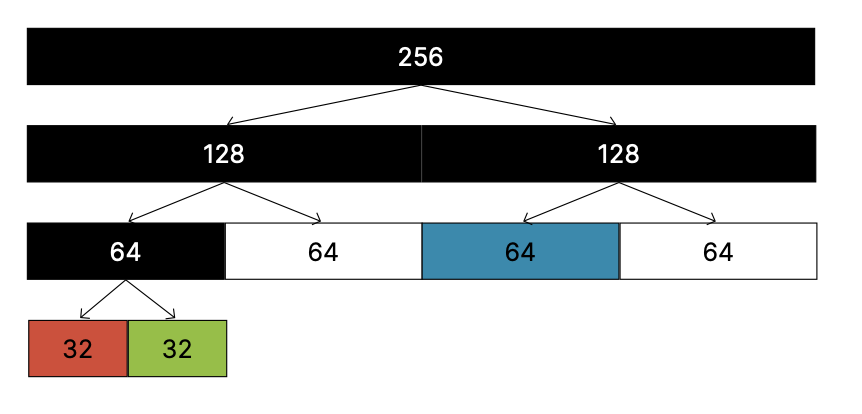
\includegraphics[width=0.8\linewidth]{img/image_2023-04-03-15-25-49.png}
    \caption{In this example we see the 256 byte block being split into two 128 byte blocks (buddy pair) and so forth. A request of size 28 or 32 may be fulfilled by any of the blocks of size 32}
\end{figure}

And what happens when we free the 64 byte block?

\begin{figure}[H]
    \centering
    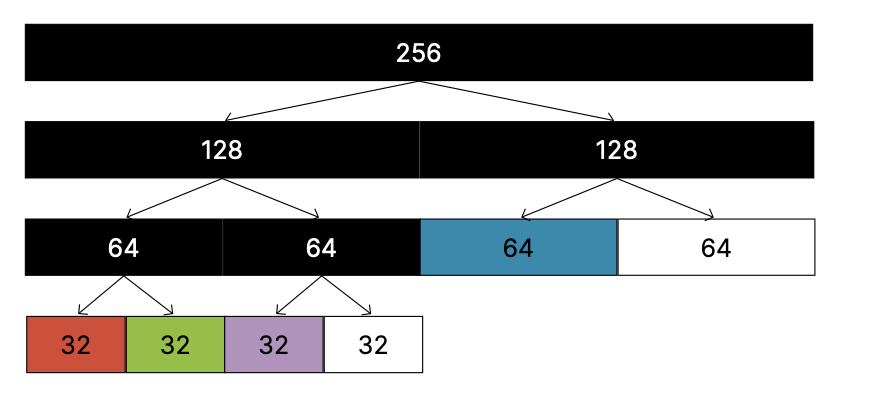
\includegraphics[width=0.8\linewidth]{img/image_2023-04-03-15-27-12.png}
    \caption{Before freeing size 64}
\end{figure}

\begin{figure}[H]
    \centering
    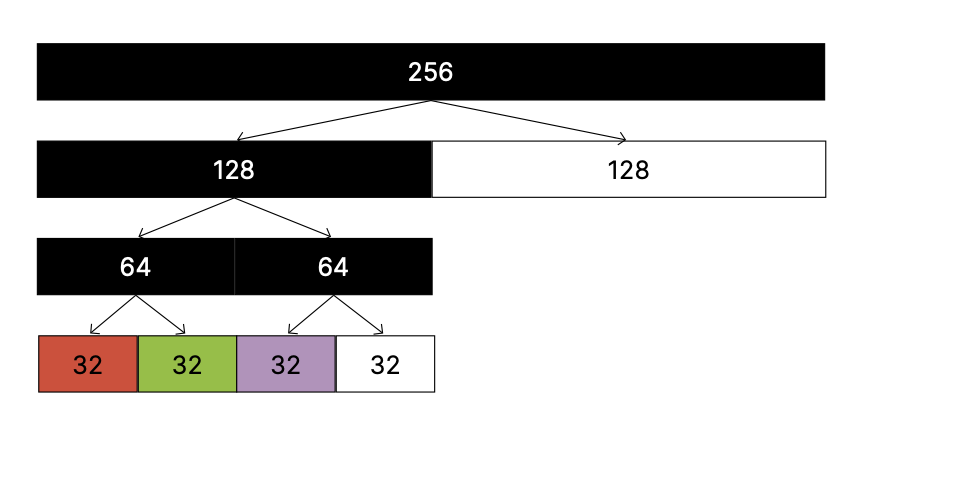
\includegraphics[width=0.8\linewidth]{img/image_2023-04-03-15-27-20.png}
    \caption{After freeing the size 64 block}
\end{figure}

Buddy allocators are extremely common and are used in the Linux kernel as well.
They are fast and simple compared to generally dynamic allocation, and avoids external fragmentation by keeping free physical pages contiguous. However it can suffer from internal fragmentation due to the rounding up of allocation size.



\subsubsection{Slab Allocators}

Slab allocators take advantage of fixed size allocations by allocating objects of the same size from a dedicated pool.
Every object type has its own pool with blocks of the correct size, preventing internal fragmentation.
It can be though of as a cache of slots\mn{Think of the ext2 filesystem we implemented in lab 6 where we have memory (blocks) and bitmaps to track which ones are free or not}


A hybrid scheme may be made by combining buddy allocation with slab allocation. This is done by allocating a slab of objects from the buddy allocator, and then allocating objects from the slab via the slab allocator.


\begin{figure}[H]
    \centering
    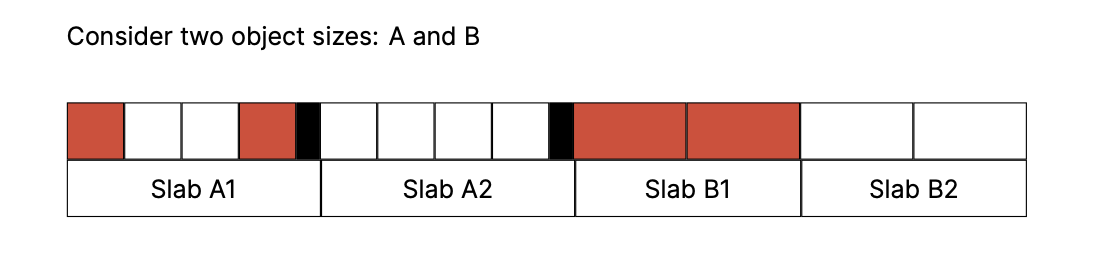
\includegraphics[width=0.8\linewidth]{img/image_2023-04-03-15-32-17.png}
    \caption{The buddy allocator allocates a slab of objects for the slab allocator to use. Here we have allocated two blocks each for objects of size A and B. Then the slab allocator manages the slabs, minimizing internal fragmentation}
\end{figure}



\end{document}
